%%%%%%%%%%%%%%%%%%%%%%%%%%%%%%%%%%%%%%%%%
% Beamer Presentation
% LaTeX Template
% Version 1.0 (10/11/12)
%
% This template has been downloaded from:
% http://www.LaTeXTemplates.com
%
% License:
% CC BY-NC-SA 3.0 (http://creativecommons.org/licenses/by-nc-sa/3.0/)
%
%%%%%%%%%%%%%%%%%%%%%%%%%%%%%%%%%%%%%%%%%

%----------------------------------------------------------------------------------------
%	PACKAGES AND THEMES
%----------------------------------------------------------------------------------------

\documentclass{beamer}

\mode<presentation> {

% The Beamer class comes with a number of default slide themes
% which change the colors and layouts of slides. Below this is a list
% of all the themes, uncomment each in turn to see what they look like.

%\usetheme{default}
%\usetheme{AnnArbor}
%\usetheme{Antibes}
%\usetheme{Bergen}
%\usetheme{Berkeley}
%\usetheme{Berlin}
%\usetheme{Boadilla}
% \usetheme{CambridgeUS}
%\usetheme{Copenhagen}
%\usetheme{Darmstadt}
%\usetheme{Dresden}
%\usetheme{Frankfurt}
%\usetheme{Goettingen}
%\usetheme{Hannover}
%\usetheme{Ilmenau}
%\usetheme{JuanLesPins}
%\usetheme{Luebeck}
\usetheme{Madrid}
%\usetheme{Malmoe}
%\usetheme{Marburg}
%\usetheme{Montpellier}
% \usetheme{PaloAlto}
%\usetheme{Pittsburgh}
%\usetheme{Rochester}
%\usetheme{Singapore}
%\usetheme{Szeged}
%\usetheme{Warsaw}

% As well as themes, the Beamer class has a number of color themes
% for any slide theme. Uncomment each of these in turn to see how it
% changes the colors of your current slide theme.

%\usecolortheme{albatross}
%\usecolortheme{beaver}
%\usecolortheme{beetle}
%\usecolortheme{crane}
%\usecolortheme{dolphin}
%\usecolortheme{dove}
%\usecolortheme{fly}
%\usecolortheme{lily}
%\usecolortheme{orchid}
\usecolortheme{rose}
%\usecolortheme{seagull}
%\usecolortheme{seahorse}
%\usecolortheme{whale}
%\usecolortheme{wolverine}

%\setbeamertemplate{footline} % To remove the footer line in all slides uncomment this line
%\setbeamertemplate{footline}[page number] % To replace the footer line in all slides with a simple slide count uncomment this line

%\setbeamertemplate{navigation symbols}{} % To remove the navigation symbols from the bottom of all slides uncomment this line
}

\usepackage{graphicx} % Allows including images
\graphicspath{{./fig/}}
\DeclareGraphicsExtensions{.pdf,.jpeg,.png}
\usepackage{booktabs} % Allows the use of \toprule, \midrule and \bottomrule in tables
\usepackage[numberedbib]{apacite}
\usepackage{ amssymb }

%----------------------------------------------------------------------------------------
%	TITLE PAGE
%----------------------------------------------------------------------------------------

\title[KFAC, ICML~\cite{pmlr-v37-martens15}] {
    Optimizing Neural Networks with Kronecker-factored Approximate Curvature~\cite{pmlr-v37-martens15} \\
    \vspace{5mm}
    ML Reading Group, UQ
}

\author{Vektor Dewanto} % Your name
\institute[] % Your institution as it will appear on the bottom of every slide, may be shorthand to save space
{
% Affiliation: RDL, UQ\\ % Your institution for the title page
% \medskip
% \textit{vektor.dewanto@gmail.com} % Your email address
}
\date{\today} % Date, can be changed to a custom date

\begin{document}

\begin{frame}
\titlepage % Print the title page as the first slide
\end{frame}

\begin{frame}
\frametitle{Outline} % Table of contents slide, comment this block out to remove it
\tableofcontents % Throughout your presentation, if you choose to use \section{} and \subsection{} commands, these will automatically be printed on this slide as an overview of your presentation
\end{frame}

%----------------------------------------------------------------------------------------
%	PRESENTATION SLIDES
%----------------------------------------------------------------------------------------
%%%%%%%%%%%%%%%%%%%%%%%%%%%%%%%%%%%%%%%%%%%%%%%%%%%%%%%%%%%%%%%%%%%%%%%%%%%%%%%
\section{Abstract}
\frame{\tableofcontents[currentsection, hideothersubsections]}

\begin{frame}
\frametitle{Abstract}

Problem:
\begin{itemize}
    \item for natural gradients, there is still NO way to efficiently compute
        the inverse of Fisher info matrix $F^{-1}$ (or its product with a vector, eg $\nabla h$)
\end{itemize}

Idea:
\begin{itemize}
    \item uses an efficiently invertible approximation to Fisher to compute approximation natural gradient
    \item concretely, approximate $F^{-1}$ as block diagonal or block tridiagonal matrices
\end{itemize}

Result:
\begin{itemize}
    \item much faster (fewer iterations) than SGD with momentum
\end{itemize}

\end{frame}

\begin{frame}
\frametitle{Abstract}
{\footnotesize
Left to right: \\
$\tilde{F}^{-1}$, its approximations $\breve{F}^{-1}$ (top) and $\hat{F}^{-1}$ (bottom), their absolute difference
}
\begin{figure}
    \centering
    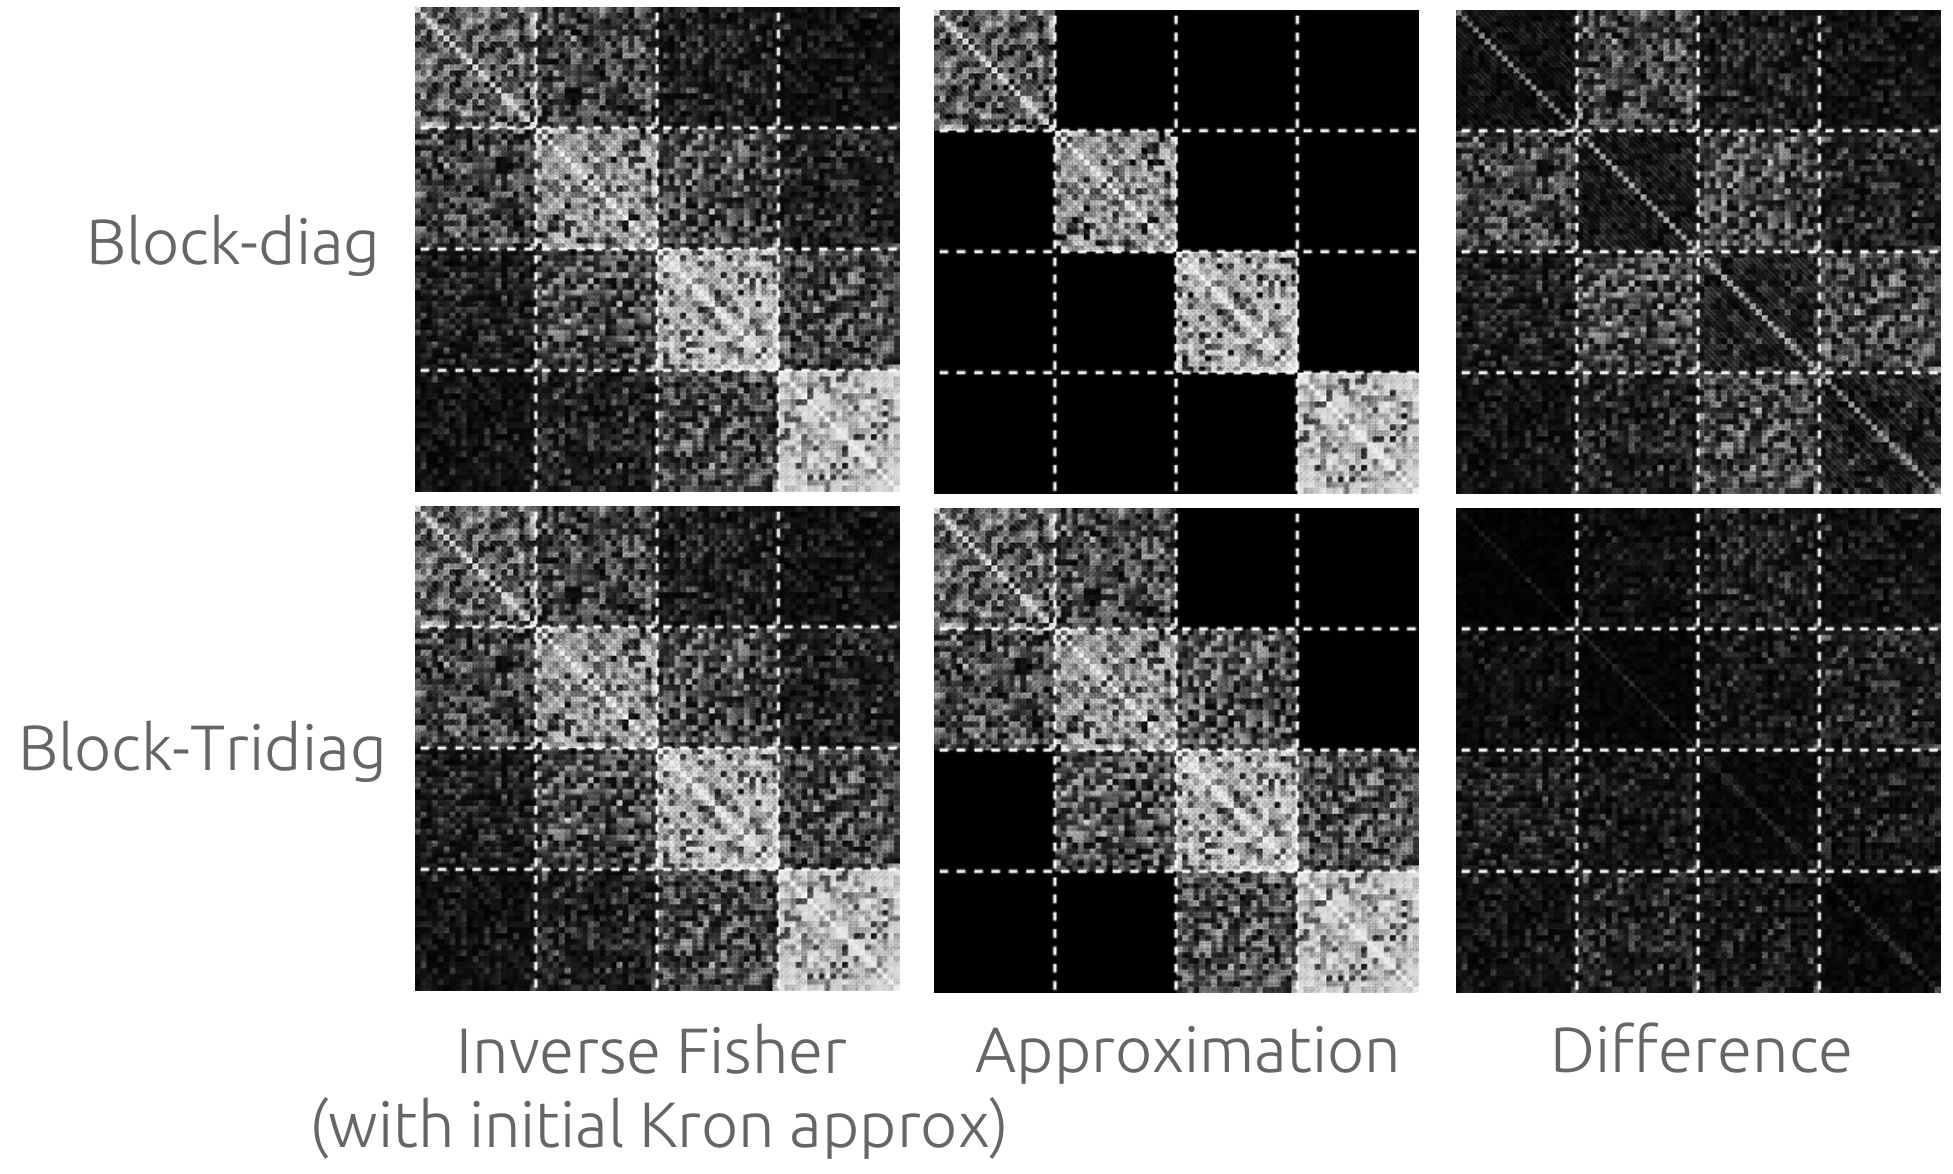
\includegraphics[scale=0.225]{kfac_12}
\end{figure}
\end{frame}

\begin{frame}
\frametitle{Abstract}
\begin{figure}
    \centering
    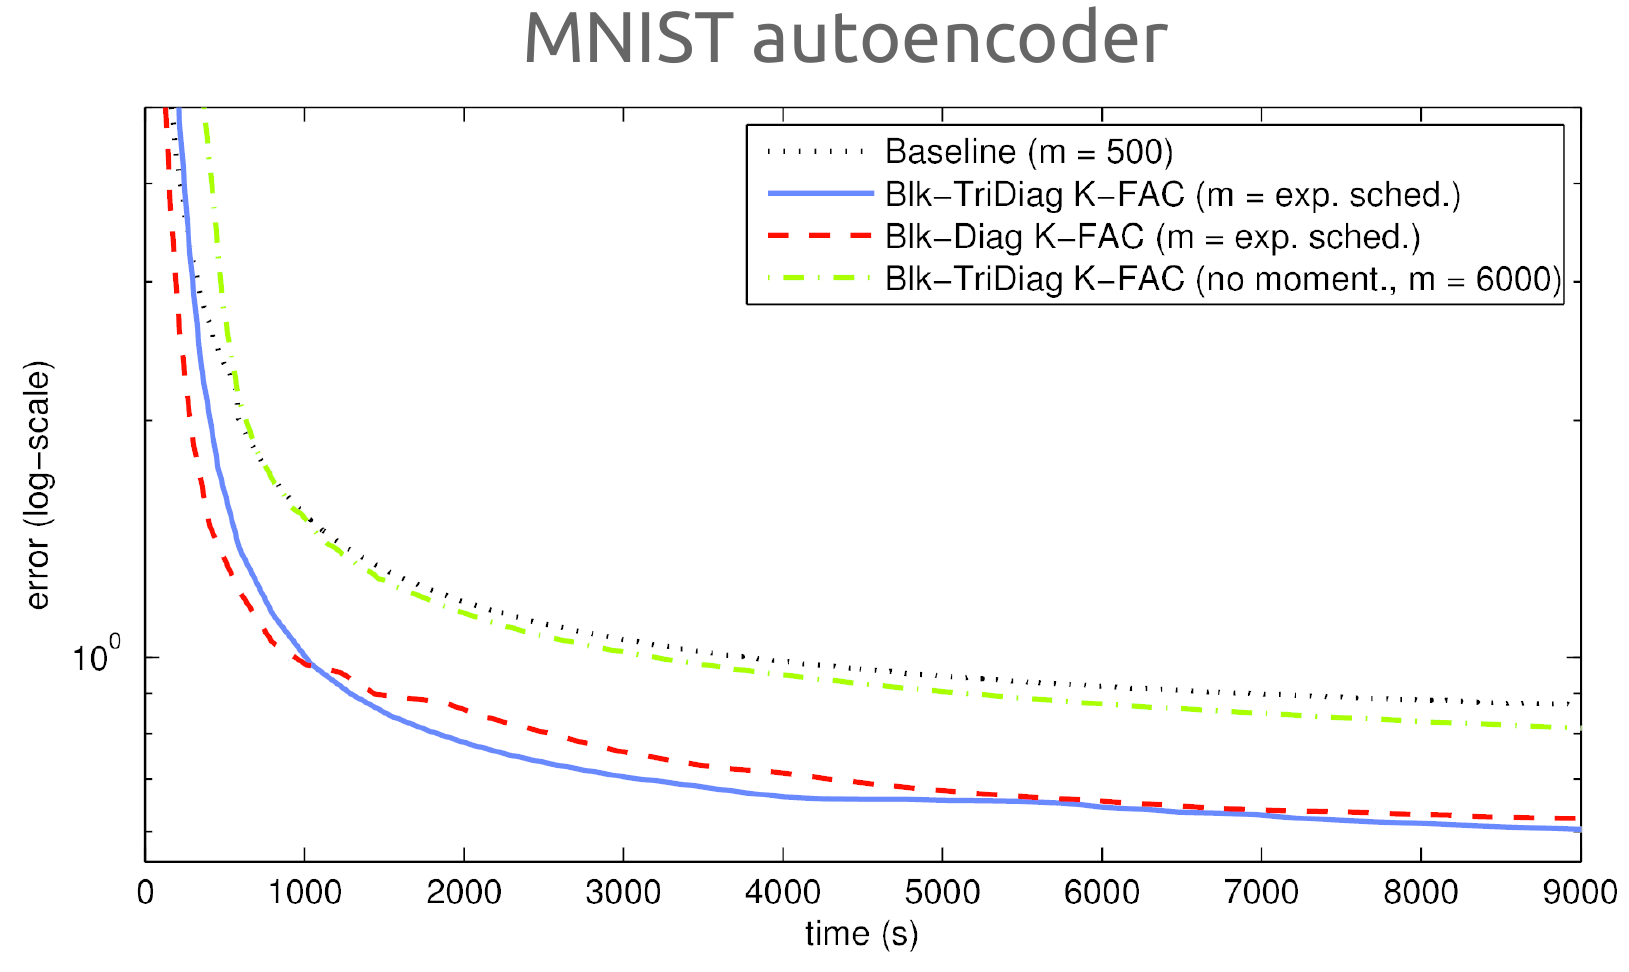
\includegraphics[scale=0.25]{mnist_autoencoder}
\end{figure}
\end{frame}

\section{Introduction}
\frame{\tableofcontents[currentsection, hideothersubsections]}

\begin{frame}
\frametitle{Introduction}

\begin{figure}
    \centering
    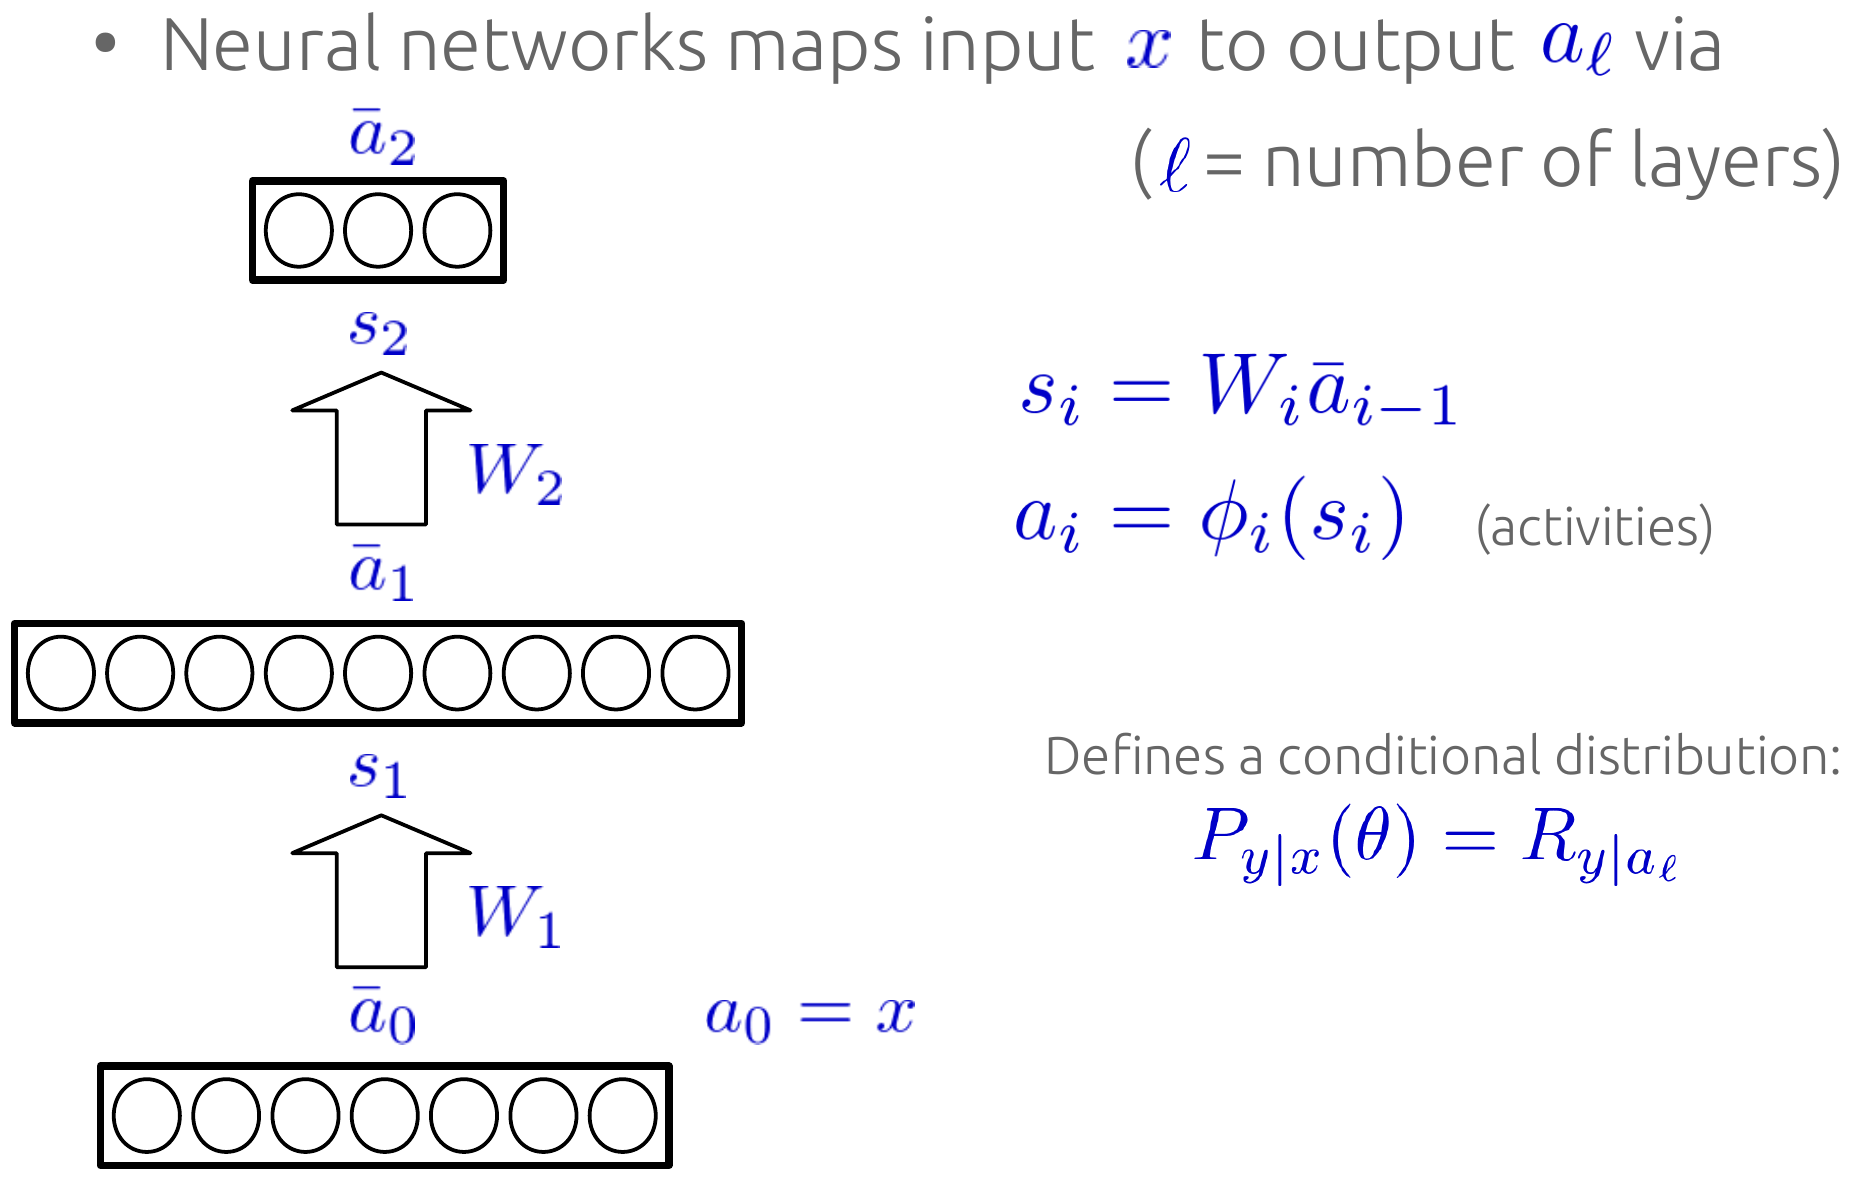
\includegraphics[scale=0.2]{net}
\end{figure}

\begin{itemize}
    \item $\bar{a}_i$ is $a_i$ appended by a homogeneous coordinate with value 1, ie
            to capture bias parameters explicitly
\end{itemize}
\end{frame}

\begin{frame}
\frametitle{Introduction}

\begin{figure}
    \centering
    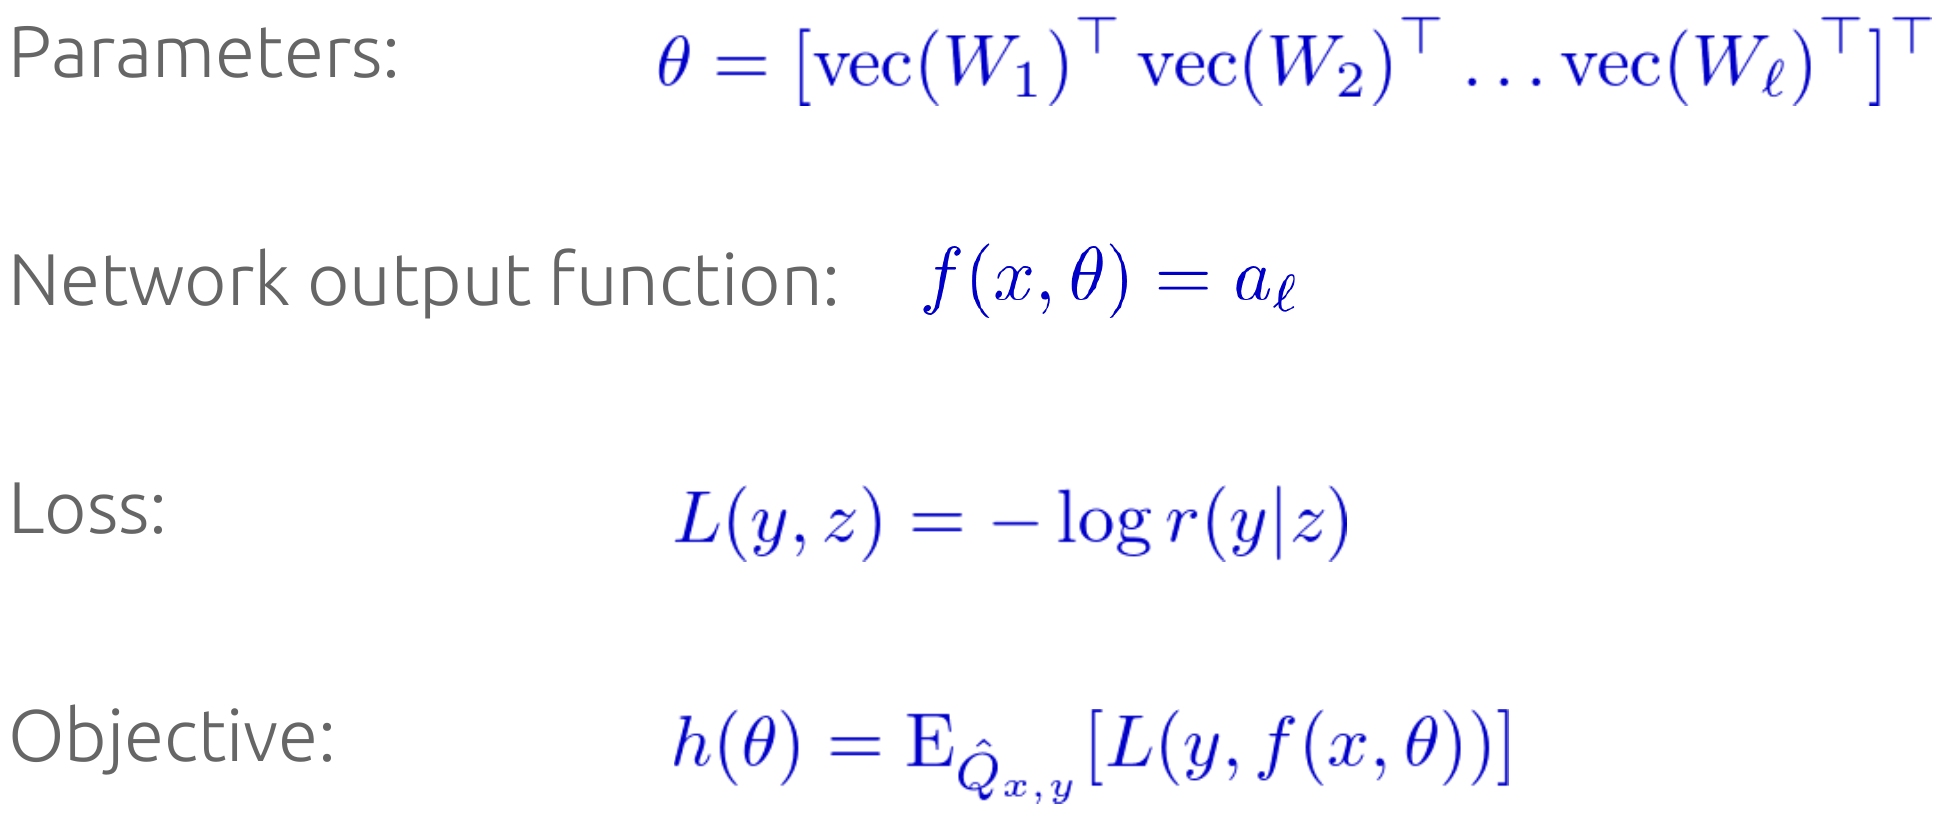
\includegraphics[scale=0.2]{net_param}
\end{figure}

\begin{itemize}
    \item $vec$ vectorizes matrices by stacking their columns together
    \item $\hat{Q}_{x, y}$ is a training distribution
    \item $p(y|x, \theta) = r(y|f(x, \theta))$ is the density function of $P_{y|x}(\theta) = R_{y|f(x,\theta)}$
    \item minimizing $h(\theta)$ can be seen as maximum likelihood learning of~$P_{y|x}(\theta)$.
\end{itemize}

\end{frame}

\begin{frame}
\frametitle{Introduction}
Newton-type update: $\theta_{k+1} = \theta_k - \alpha_k (\nabla^2 h)^{-1} \nabla h$
% \begin{itemize}
%     \item Newton-type update: $\theta_{t+1} = \theta_t - \alpha (\nabla^2 h)^{-1} \nabla h$
% \end{itemize}
\begin{figure}
    \raggedright
    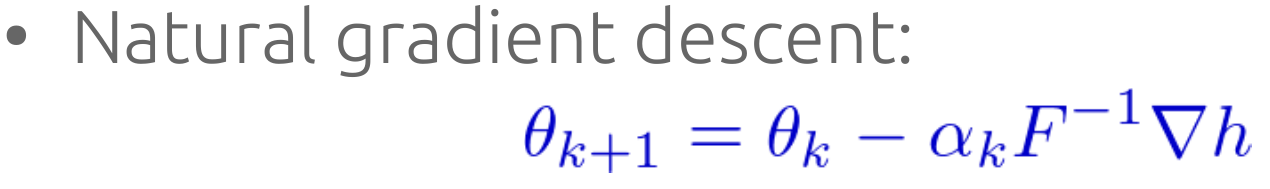
\includegraphics[scale=0.25]{natgrad}
\end{figure}

\begin{figure}
    \raggedright
    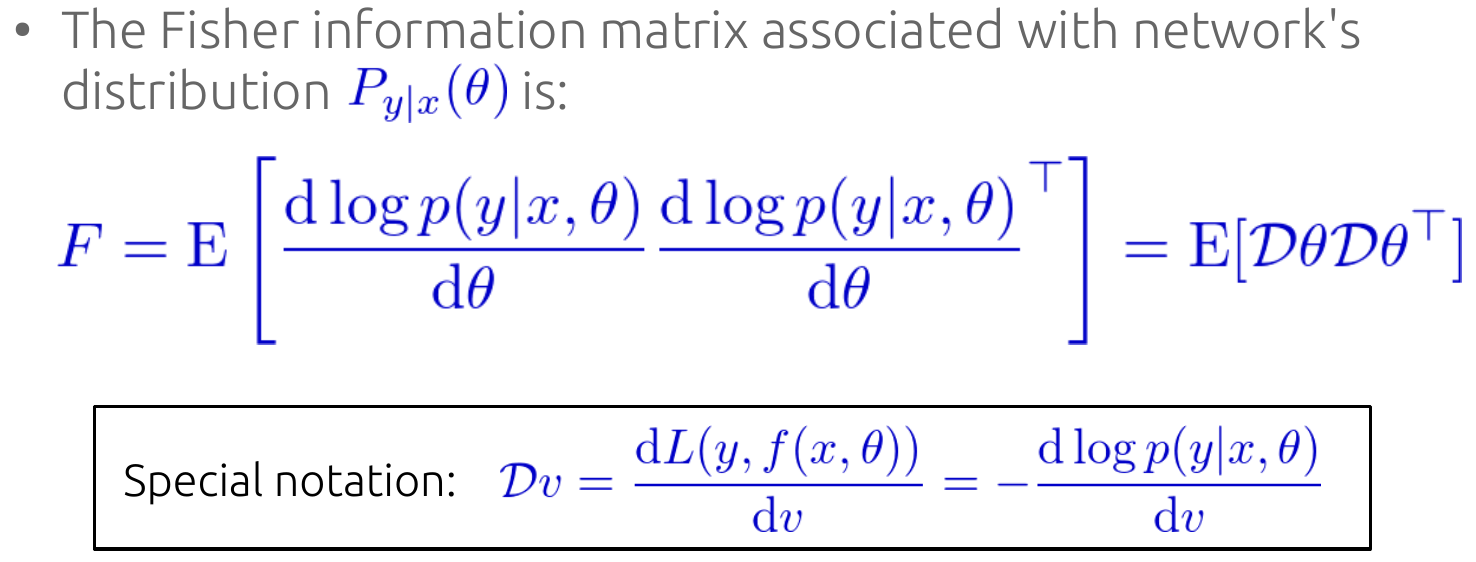
\includegraphics[scale=0.25]{fisher}
\end{figure}

\end{frame}

\section{KFAC: initial approximation $\tilde{F} \approx F$}
\frame{\tableofcontents[currentsection, hideothersubsections]}

\begin{frame}
\frametitle{KFAC: Initial approximation $\tilde{F} \approx F$}

Recall:
\begin{figure}
    \raggedright
    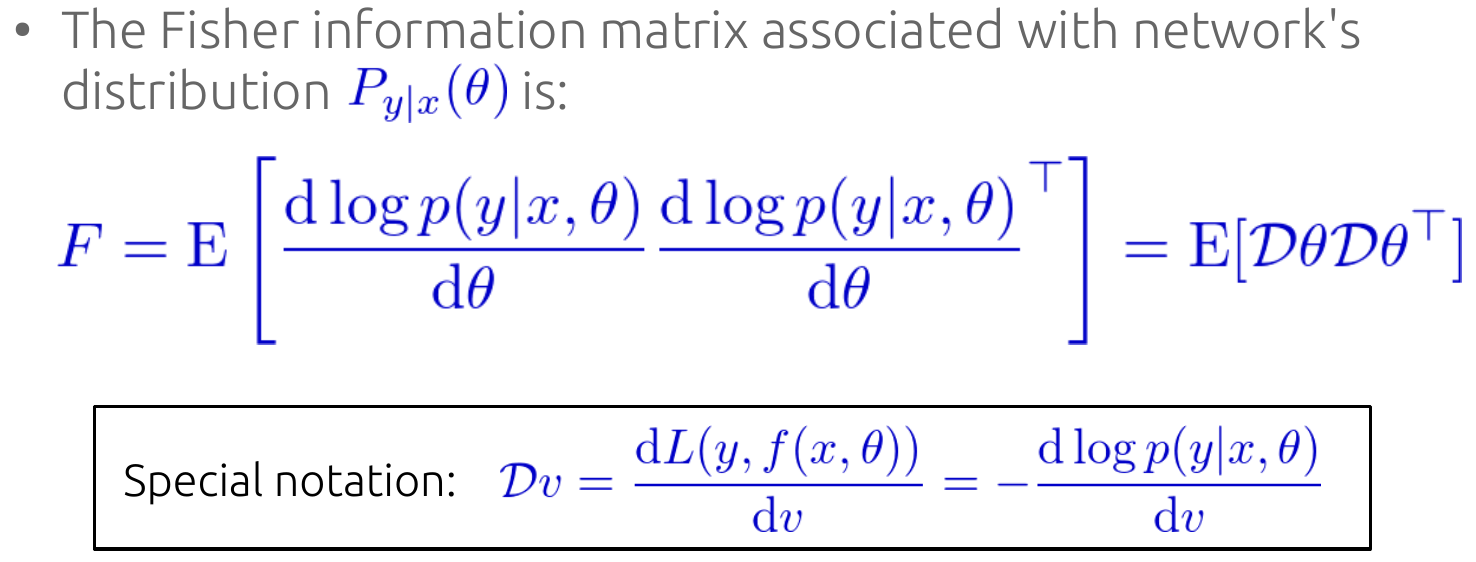
\includegraphics[scale=0.25]{fisher}
\end{figure}

\end{frame}

\begin{frame}
\frametitle{KFAC: Initial approximation $\tilde{F} \approx F$}

\begin{figure}
    \raggedright
    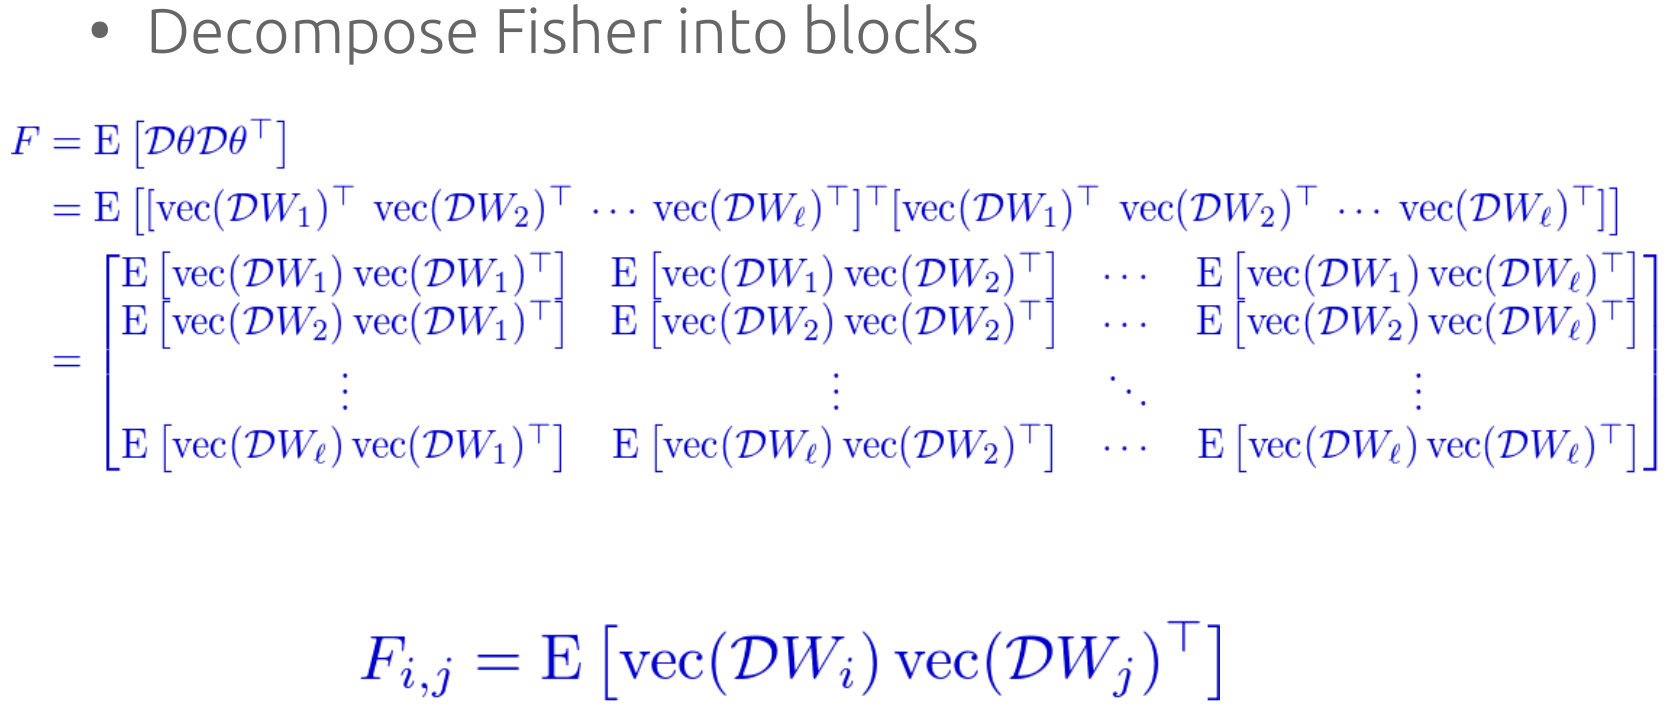
\includegraphics[scale=0.25]{kfac_01}
\end{figure}

$F$ can be viewed as an $\ell$ by $\ell$ block matrix.\\
(blocks correpond to layers)
\end{frame}

\begin{frame}
\frametitle{KFAC: Initial approximation $\tilde{F} \approx F$}

$g_i = \mathcal{D}s_i$ is the derivative of the loss wrt the inputs to units at layer $i$
\begin{figure}
    \raggedright
    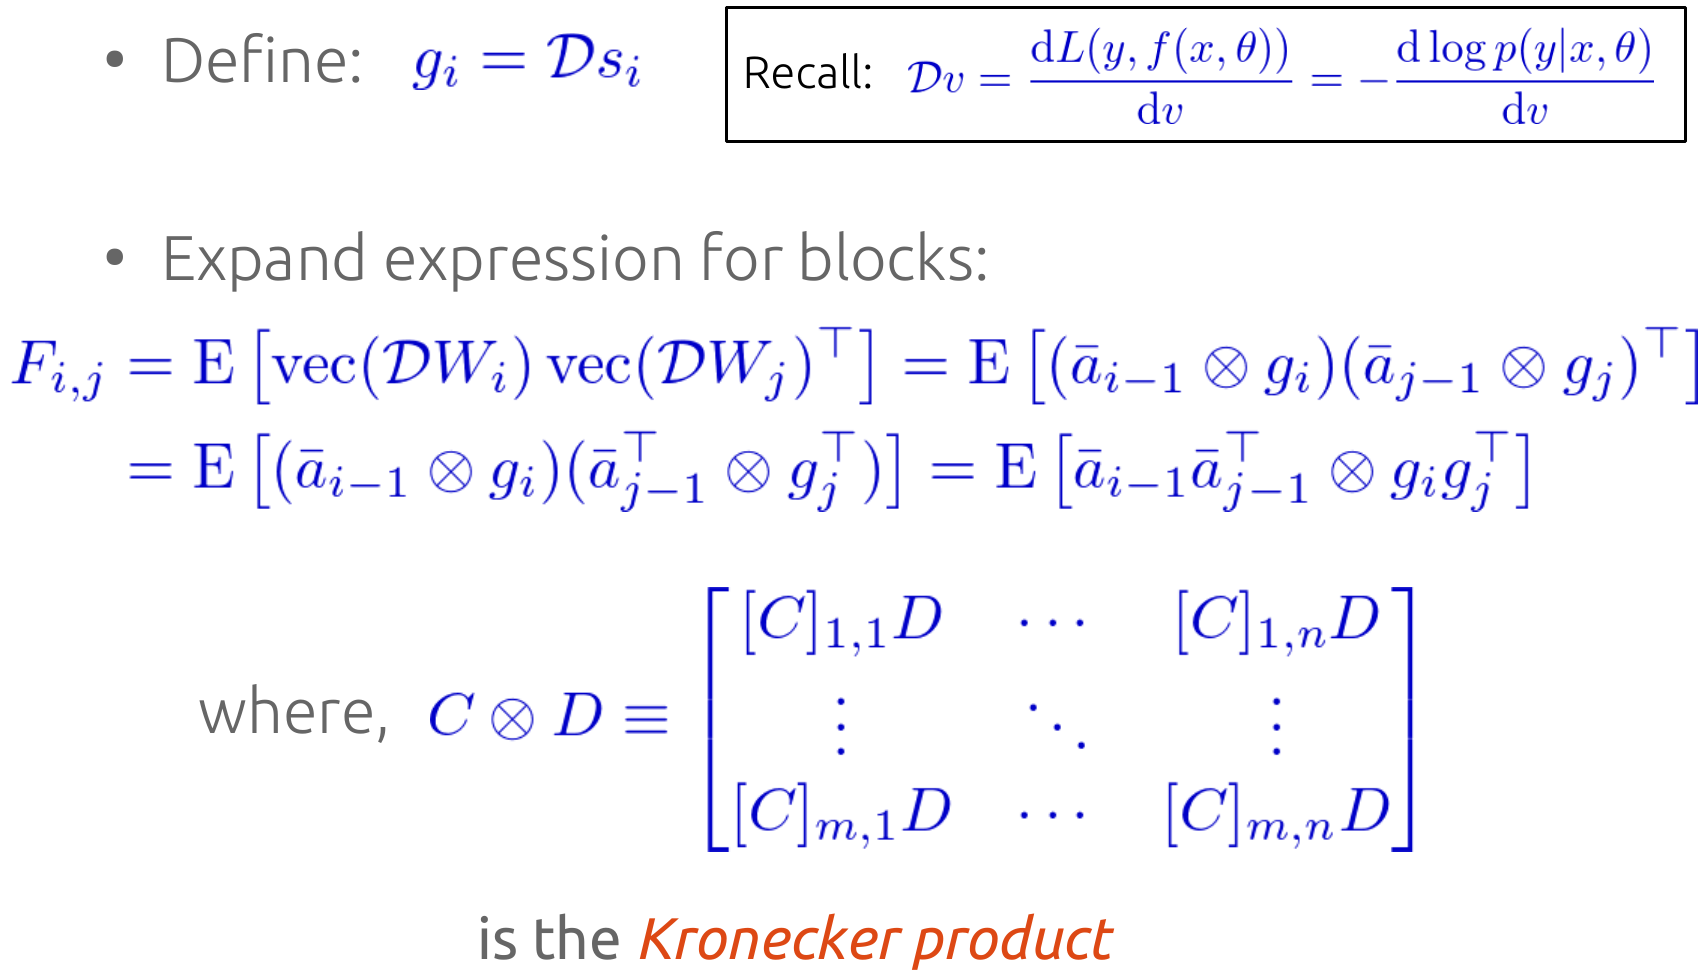
\includegraphics[scale=0.25]{kfac_02}
\end{figure}

Recall: $(A \otimes B)^T = (A^T \otimes B^T)$ and $(A \otimes B) (C \otimes D) = (AC \otimes BD)$
\end{frame}

\begin{frame}
\frametitle{KFAC: Initial approximation $\tilde{F} \approx F$}

\begin{figure}
    \raggedright
    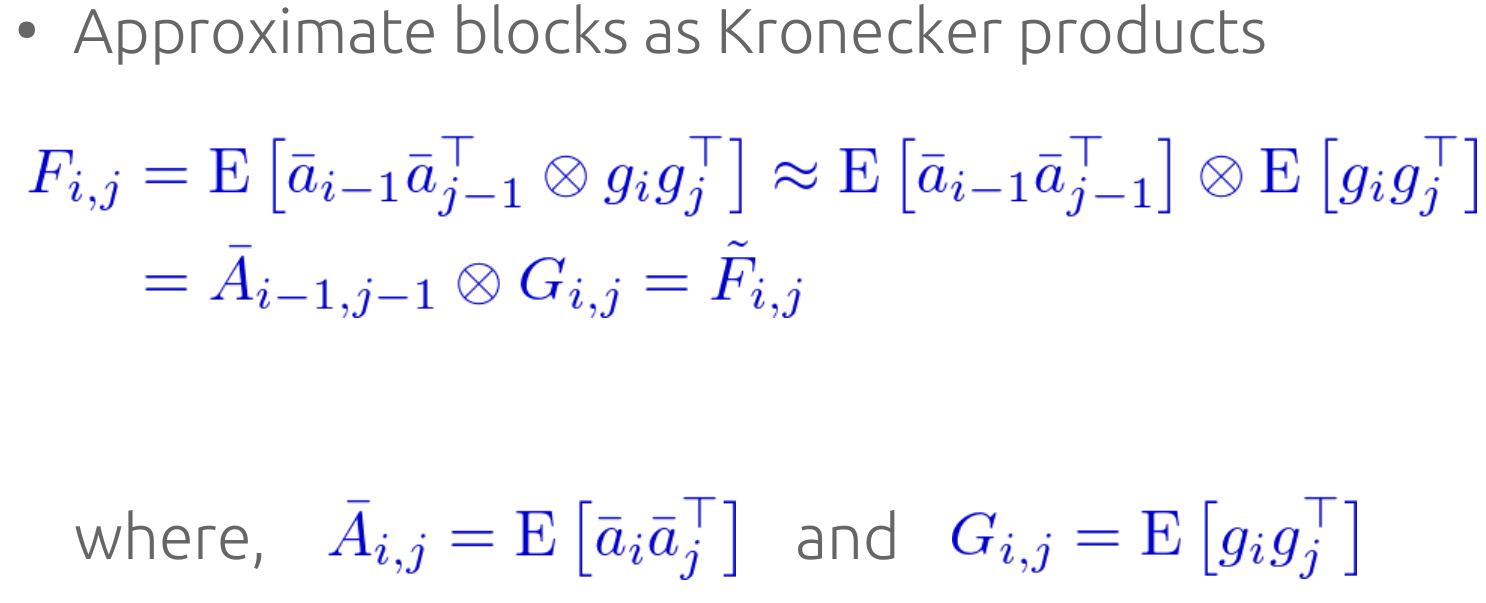
\includegraphics[scale=0.2]{kfac_03}
\end{figure}

\begin{figure}
    \raggedright
    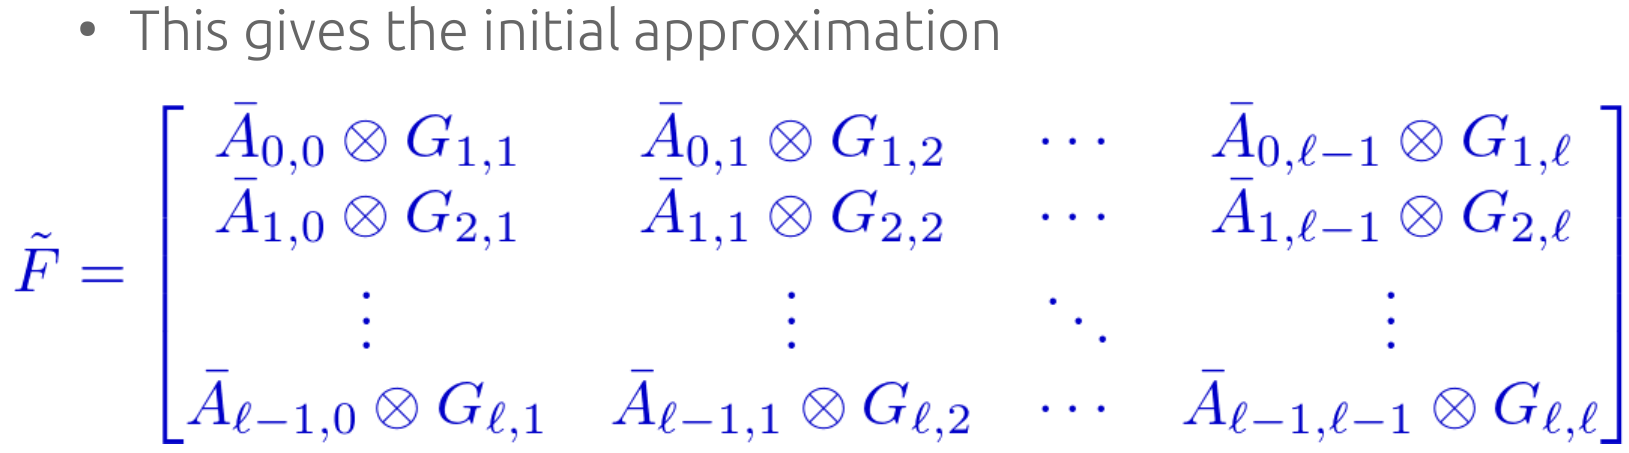
\includegraphics[scale=0.2]{kfac_04}
\end{figure}

$\tilde{F}$ is indeed a major approximation because\\
the expectation of a Kronecker product is, in general, NOT
equal to the Kronecker product of expectations

\end{frame}

\begin{frame}
\frametitle{KFAC: Initial approximation $\tilde{F} \approx F$}
Comparing the exact $F$ vs its approximate $\tilde{F}$
\begin{figure}
    \centering
    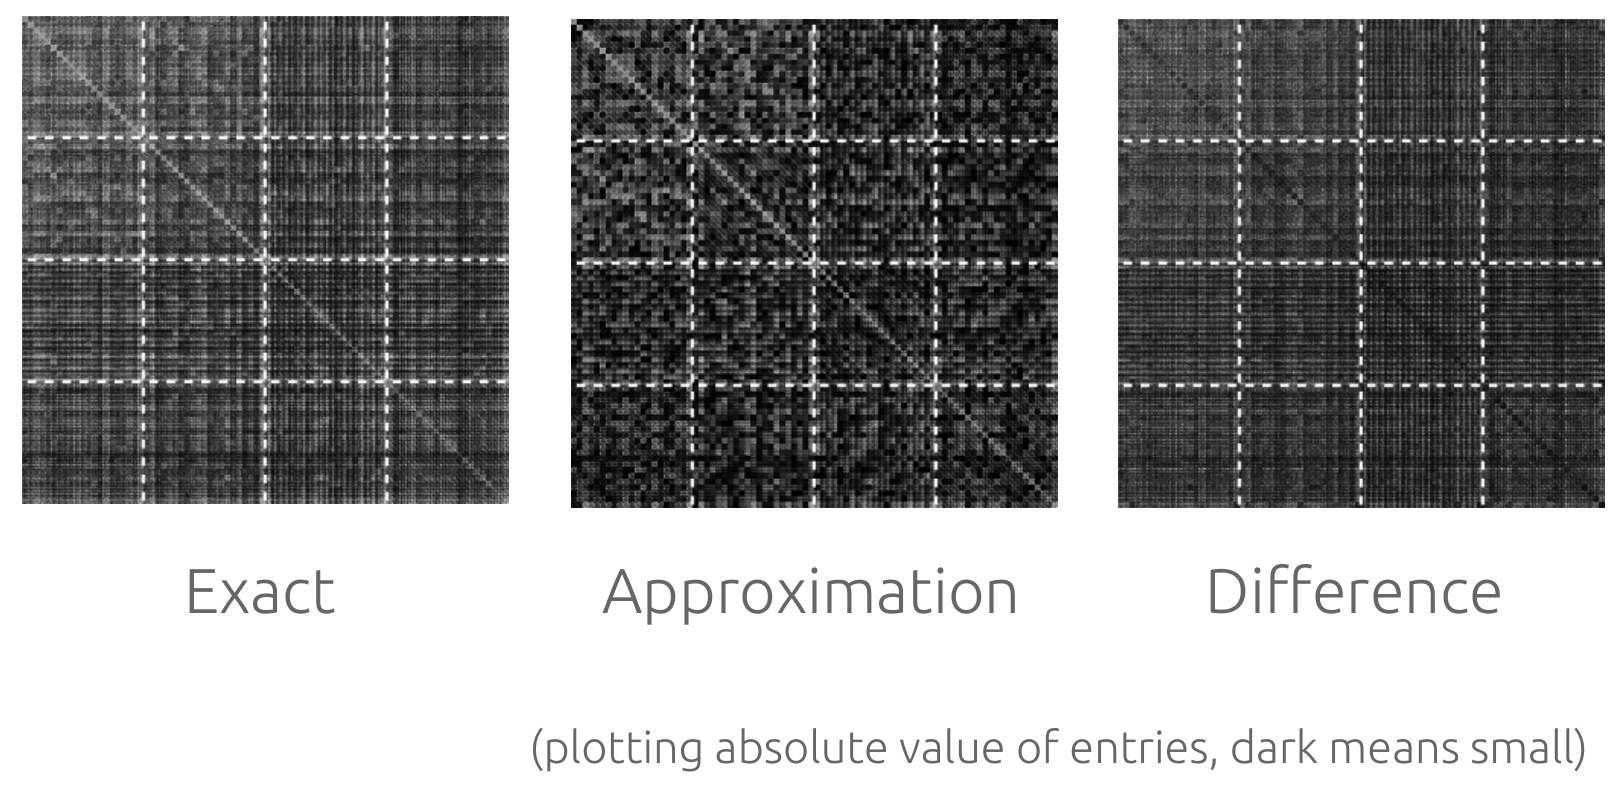
\includegraphics[scale=0.275]{kfac_05}
\end{figure}

\end{frame}

\begin{frame}
\frametitle{KFAC: Initial approximation $\tilde{F} \approx F$}
Recall:
\begin{figure}
    \raggedright
    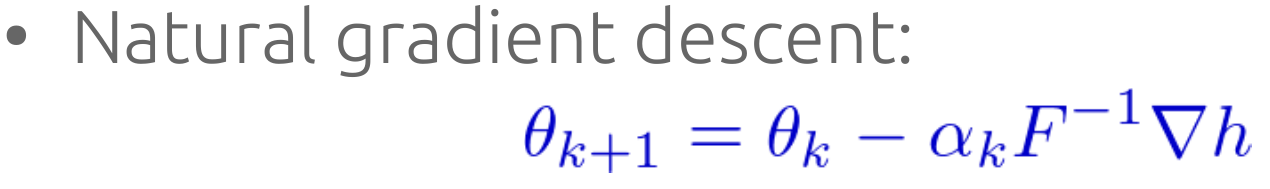
\includegraphics[scale=0.2]{natgrad}
\end{figure}

We already have $\tilde{F} \approx F$, then: \\
how to \textbf{efficiently} compute $\tilde{F}^{-1}$ or its product, $\tilde{F}^{-1}\nabla h$?
\end{frame}

\begin{frame}
\frametitle{KFAC: Initial approximation $\tilde{F} \approx F$}
Structure in the inverse Fisher:
\begin{figure}
    \centering
    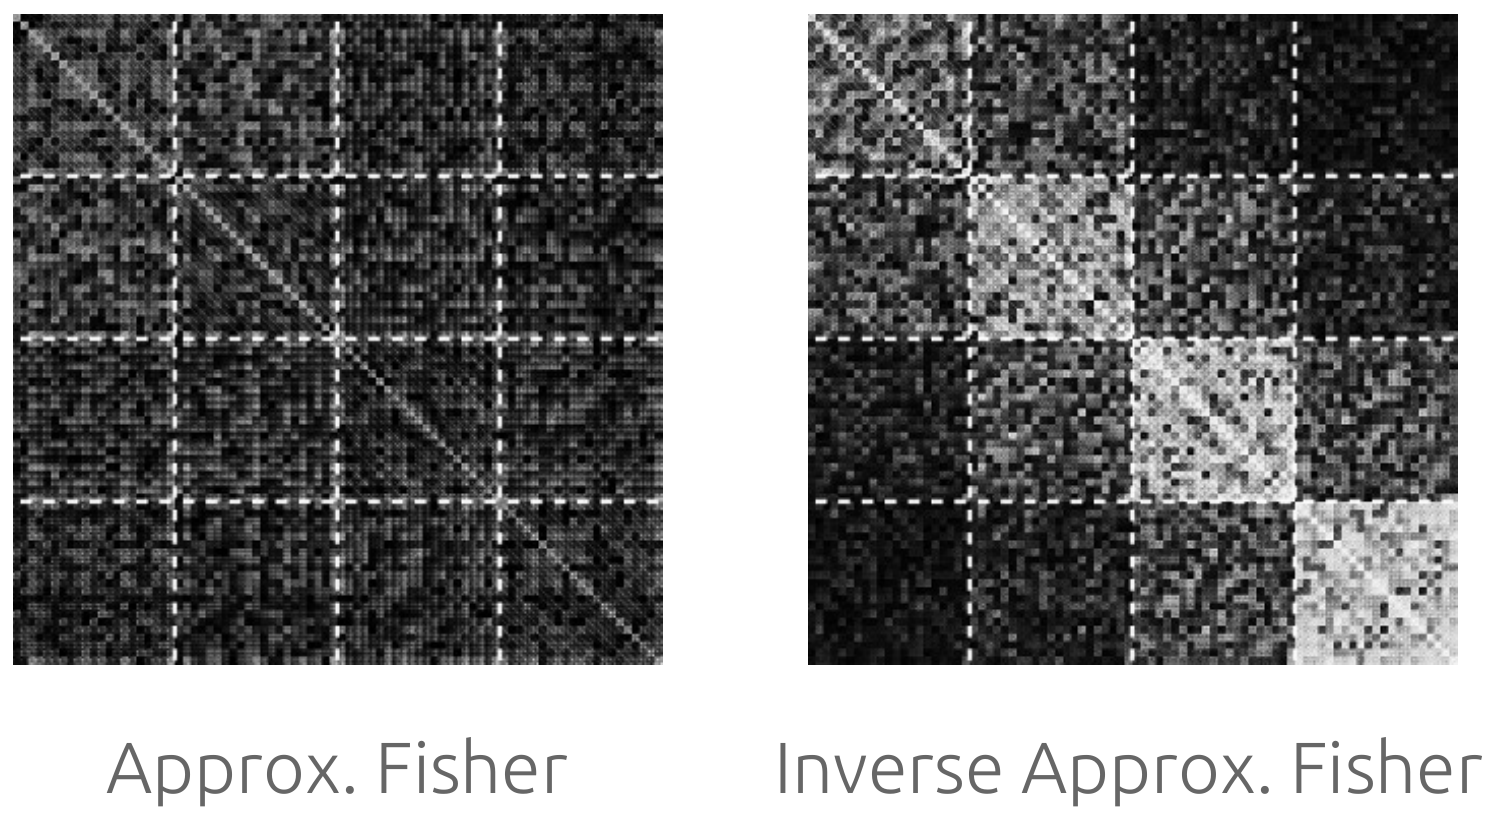
\includegraphics[scale=0.2]{kfac_06}
\end{figure}
(plotting absolute value of entries, dark means small)
\end{frame}

\begin{frame}
\frametitle{KFAC: Initial approximation $\tilde{F} \approx F$}
Based on Structured Inverses (Pourahmadi, 2011):
\begin{figure}
    \raggedright
    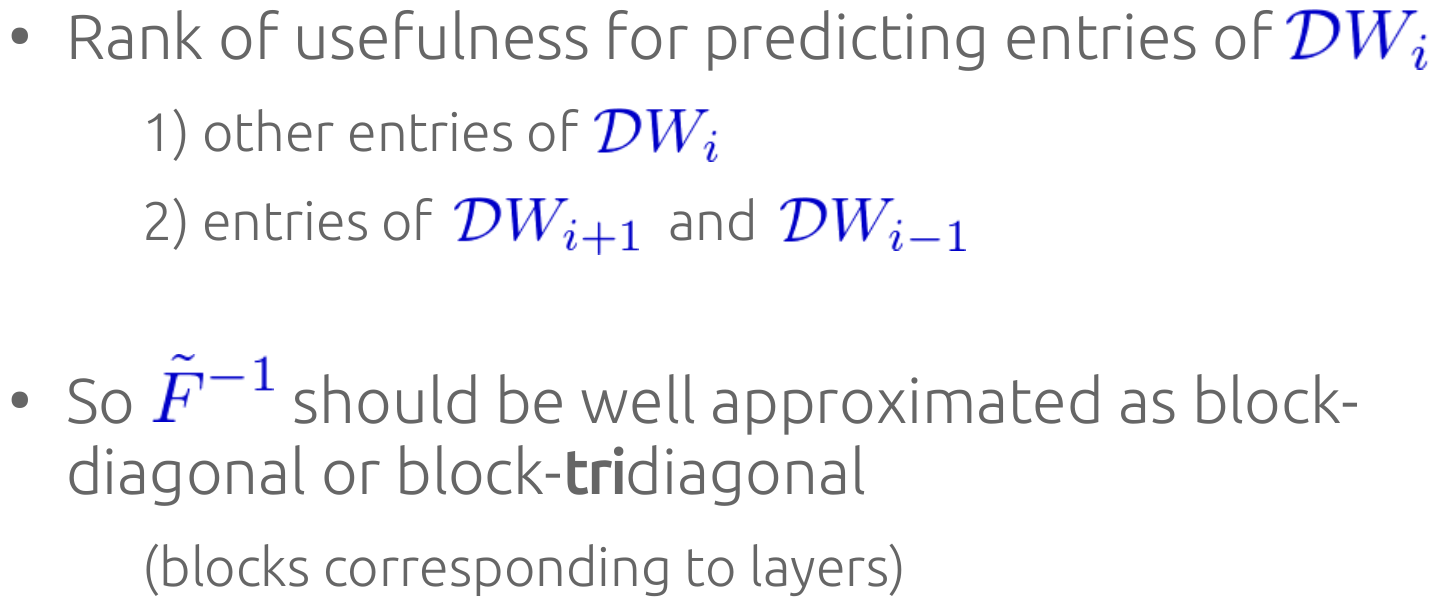
\includegraphics[scale=0.275]{kfac_07}
\end{figure}
\end{frame}

\section{KFAC: Block-diagonal inverse approx, $\breve{F}^{-1} \approx \tilde{F}^{-1}$}
\frame{\tableofcontents[currentsection, hideothersubsections]}

\begin{frame}
\frametitle{KFAC: Block-diagonal inverse approx, $\breve{F}^{-1} \approx \tilde{F}^{-1}$}
\begin{figure}
    \centering
    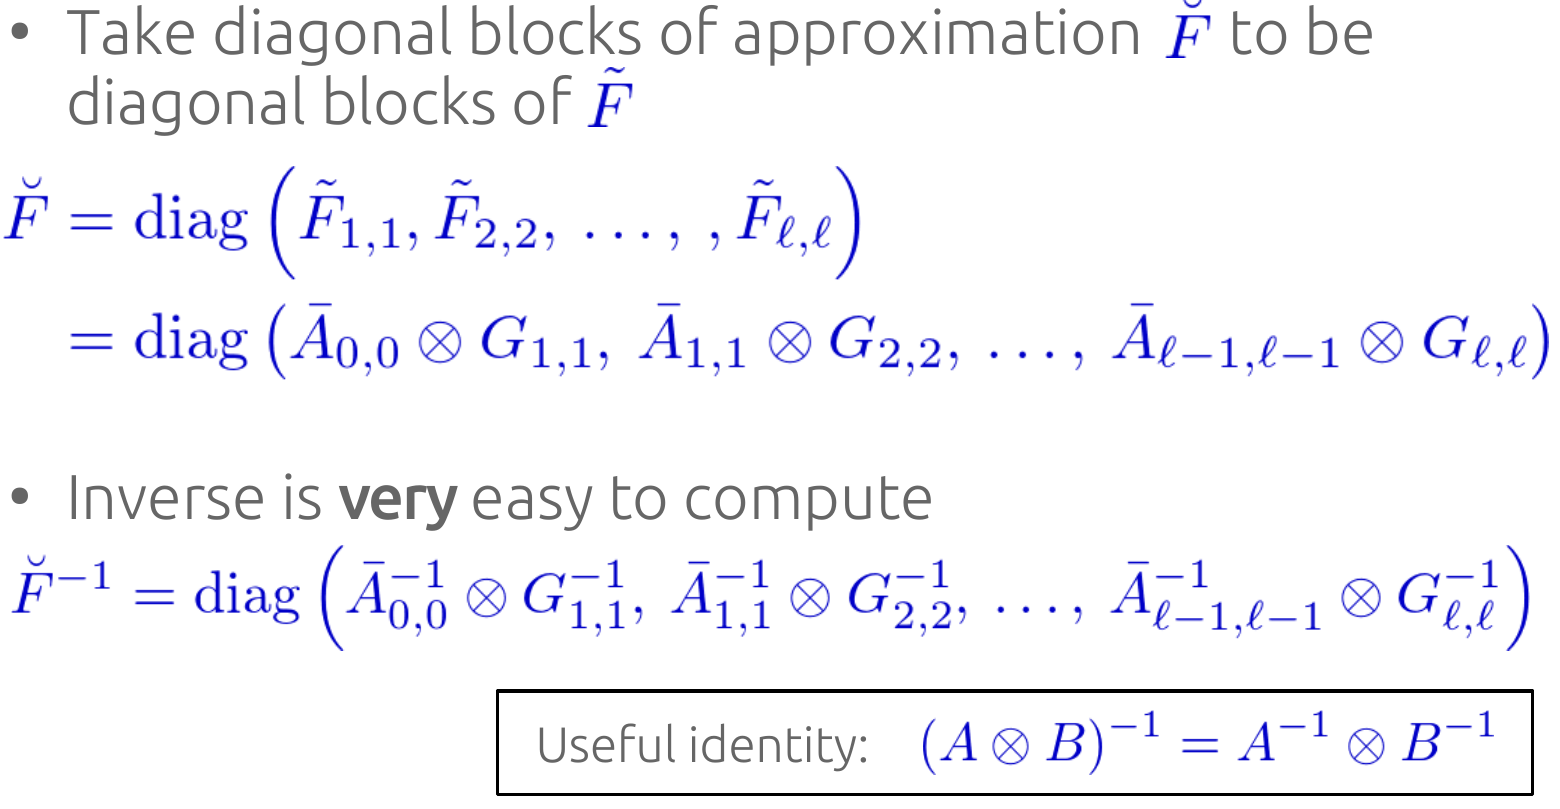
\includegraphics[scale=0.275]{kfac_08}
\end{figure}
NOTE: this is equivalent to approximating Fisher itself as block-diagonal
\end{frame}

\begin{frame}
\frametitle{KFAC: Block-diagonal inverse approx, $\breve{F}^{-1} \approx \tilde{F}^{-1}$}
\begin{figure}
    \centering
    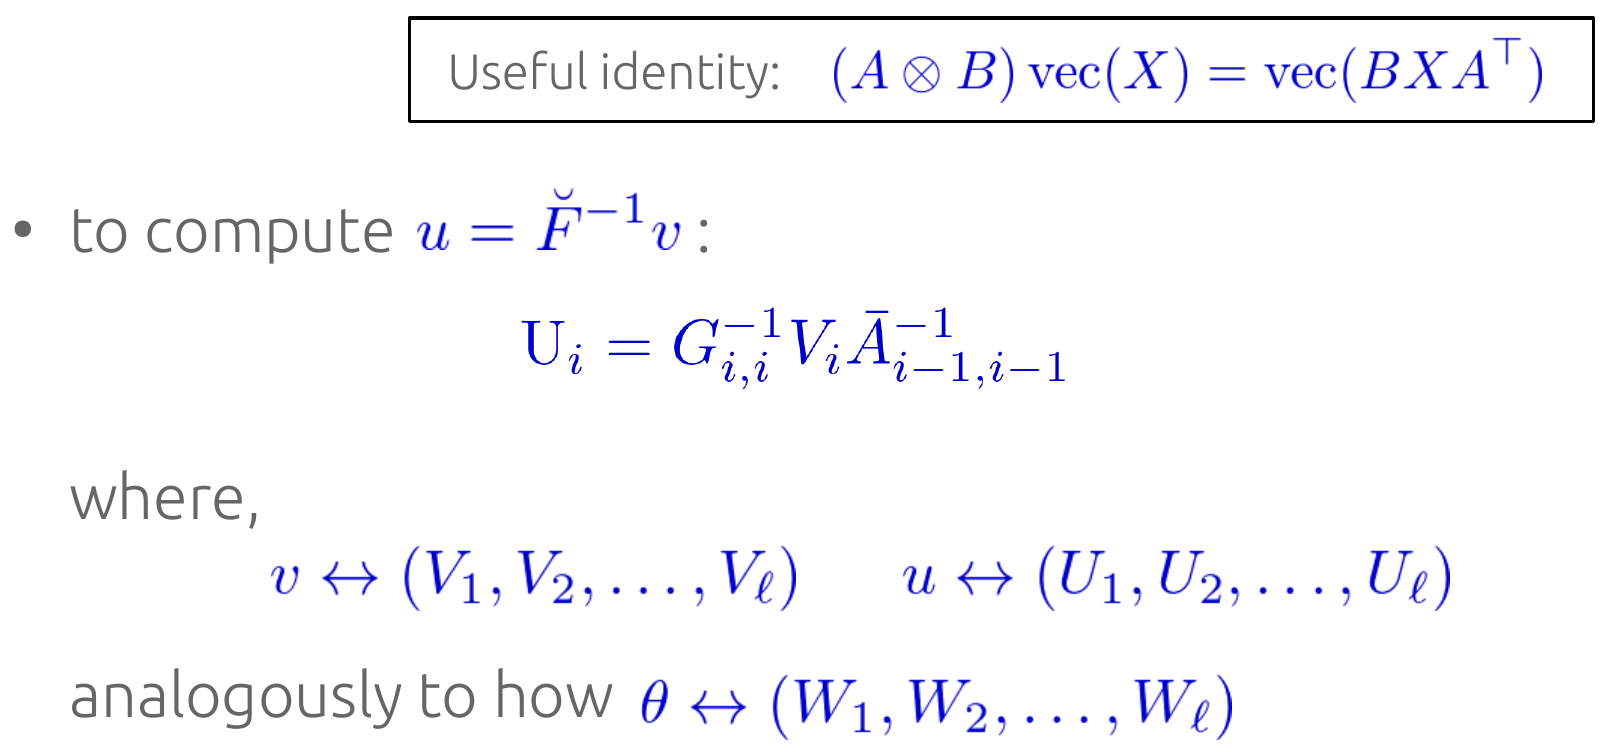
\includegraphics[scale=0.275]{kfac_09}
\end{figure}
\end{frame}

\begin{frame}
\frametitle{KFAC: Block-diagonal inverse approx, $\breve{F}^{-1} \approx \tilde{F}^{-1}$}
{\footnotesize
Left to right: \\
$\tilde{F}^{-1}$, its approximations $\breve{F}^{-1}$ (top) and $\hat{F}^{-1}$ (bottom), their absolute difference
}
\begin{figure}
    \centering
    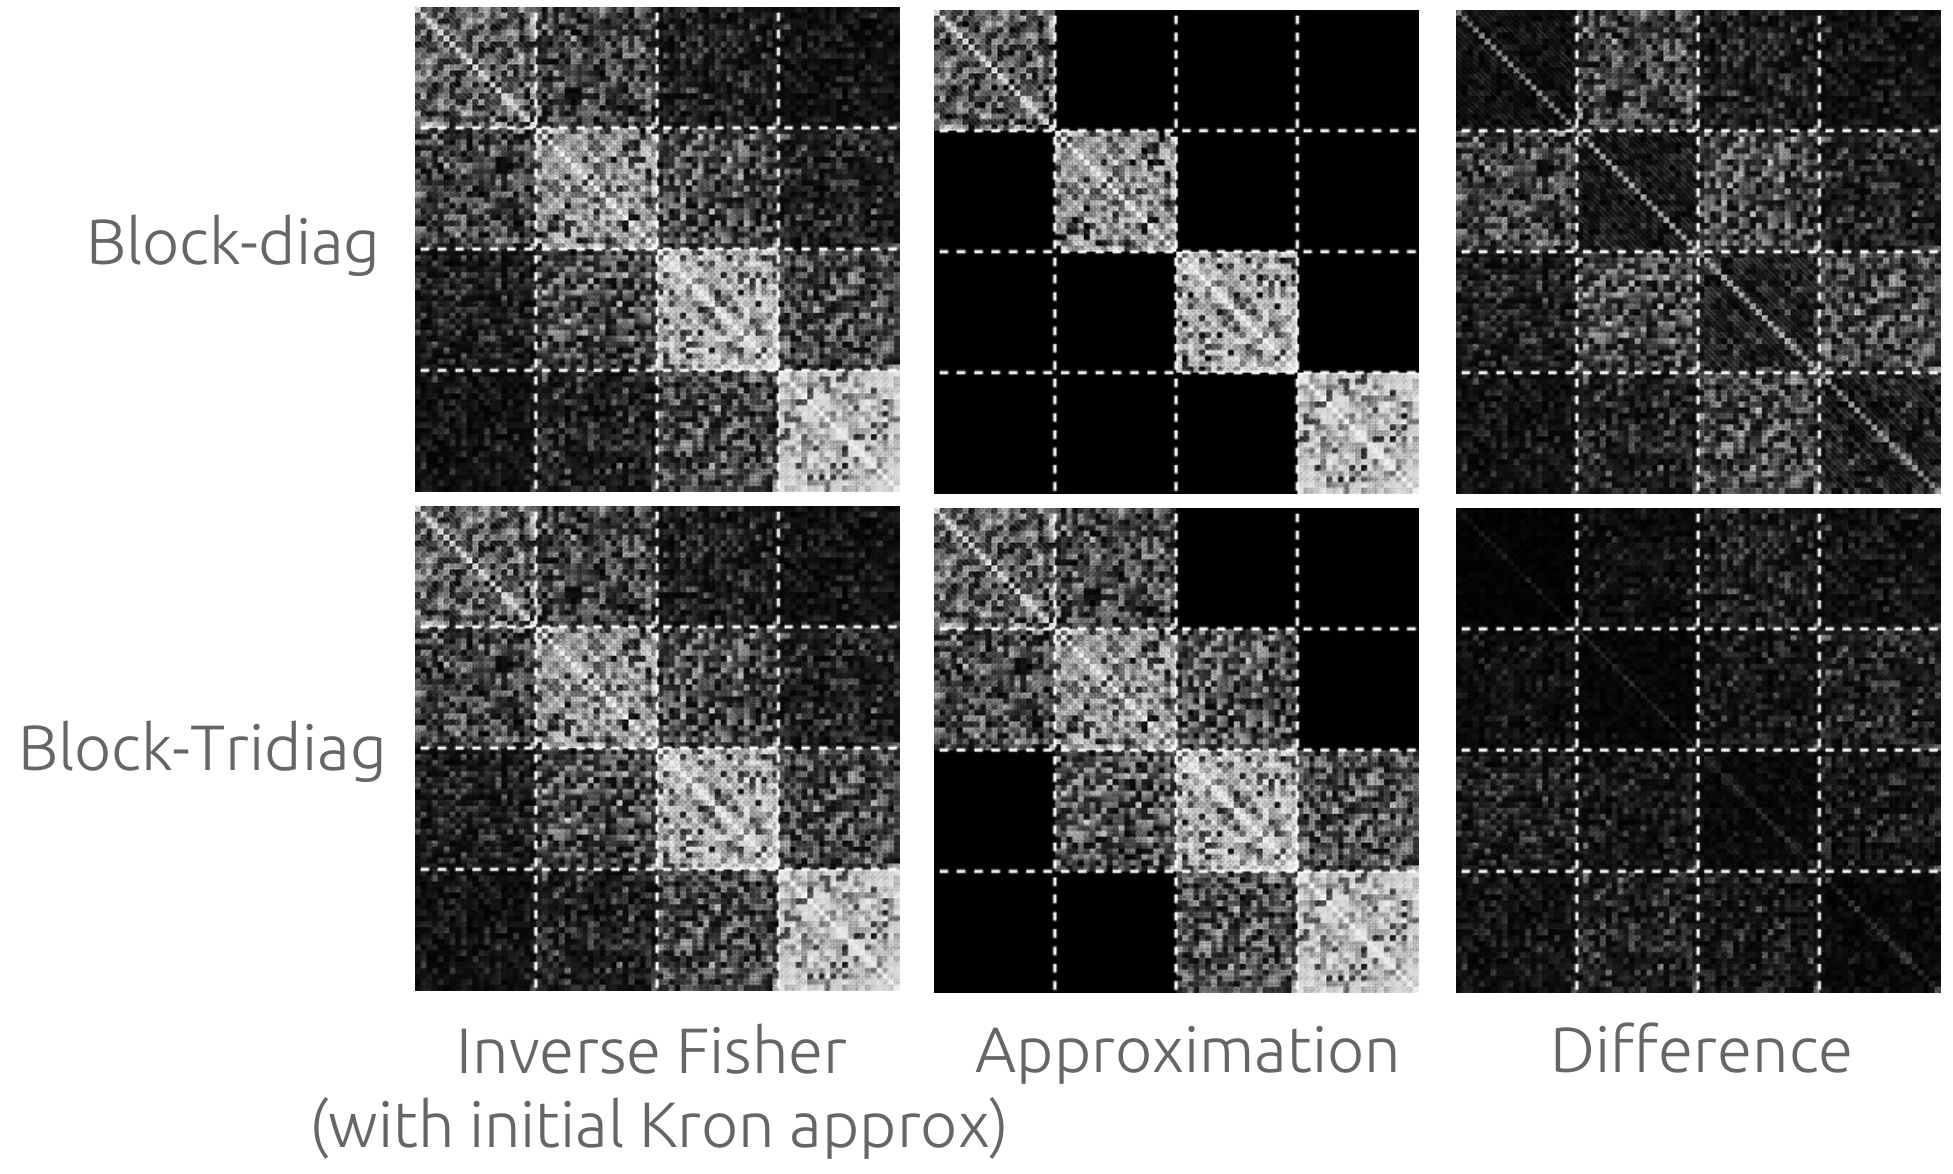
\includegraphics[scale=0.225]{kfac_12}
\end{figure}
\end{frame}

% \begin{frame}
% \frametitle{KFAC: Block-diagonal inverse approx, $\breve{F}^{-1} \approx \tilde{F}^{-1}$}
% Left to right: \\
% $\tilde{F}$, its approximations $\breve{F}$ (top) and $\hat{F}$ (bottom), their absolute difference

% \begin{figure}
%     \centering
%     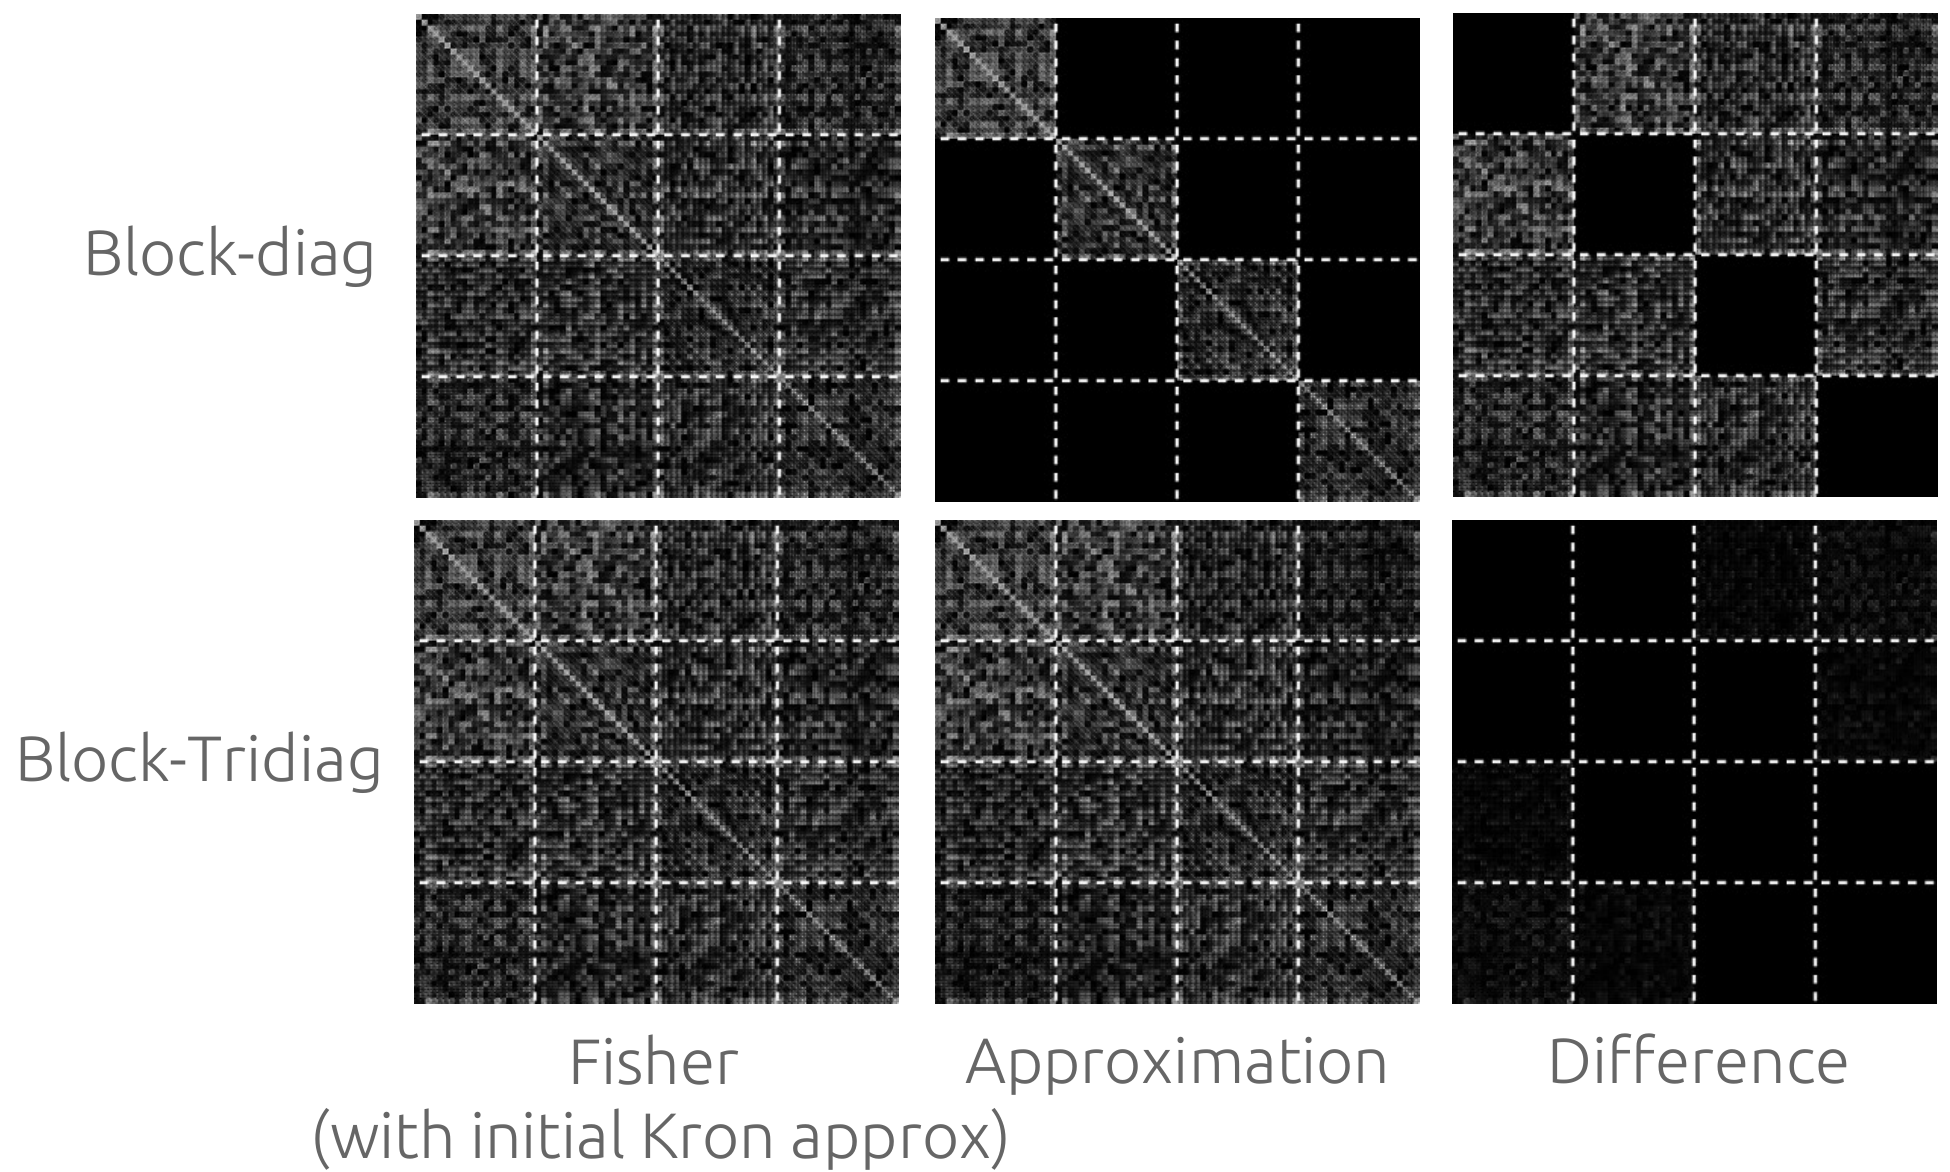
\includegraphics[scale=0.175]{kfac_10}
% \end{figure}

% \begin{itemize}
%     \item the off-tridiagonal blocks of the bottom right matrix, while being very close to zero, are
%     actually NON-zero (hard to see from the plot)
%     % \item the plot is of the absolute values of the entries
% \end{itemize}
% \end{frame}

\section{KFAC: Block-tridiagonal inverse approx, $\hat{F}^{-1} \approx \tilde{F}^{-1}$}
\frame{\tableofcontents[currentsection, hideothersubsections]}

\begin{frame}
\frametitle{KFAC: Block-tridiagonal inverse approx, $\hat{F}^{-1} \approx \tilde{F}^{-1}$}
Likely, tridiagonal approx $\hat{F}^{-1}$ is better than (one)diagonal $\breve{F}^{-1}$,
BUT harder to obtain because\\
approximating $\tilde{F}^{-1}$ as block-tridiagonal is NOT equivalent to approximating $\tilde{F}$ as block-tridiagonal.

\begin{figure}
    \centering
    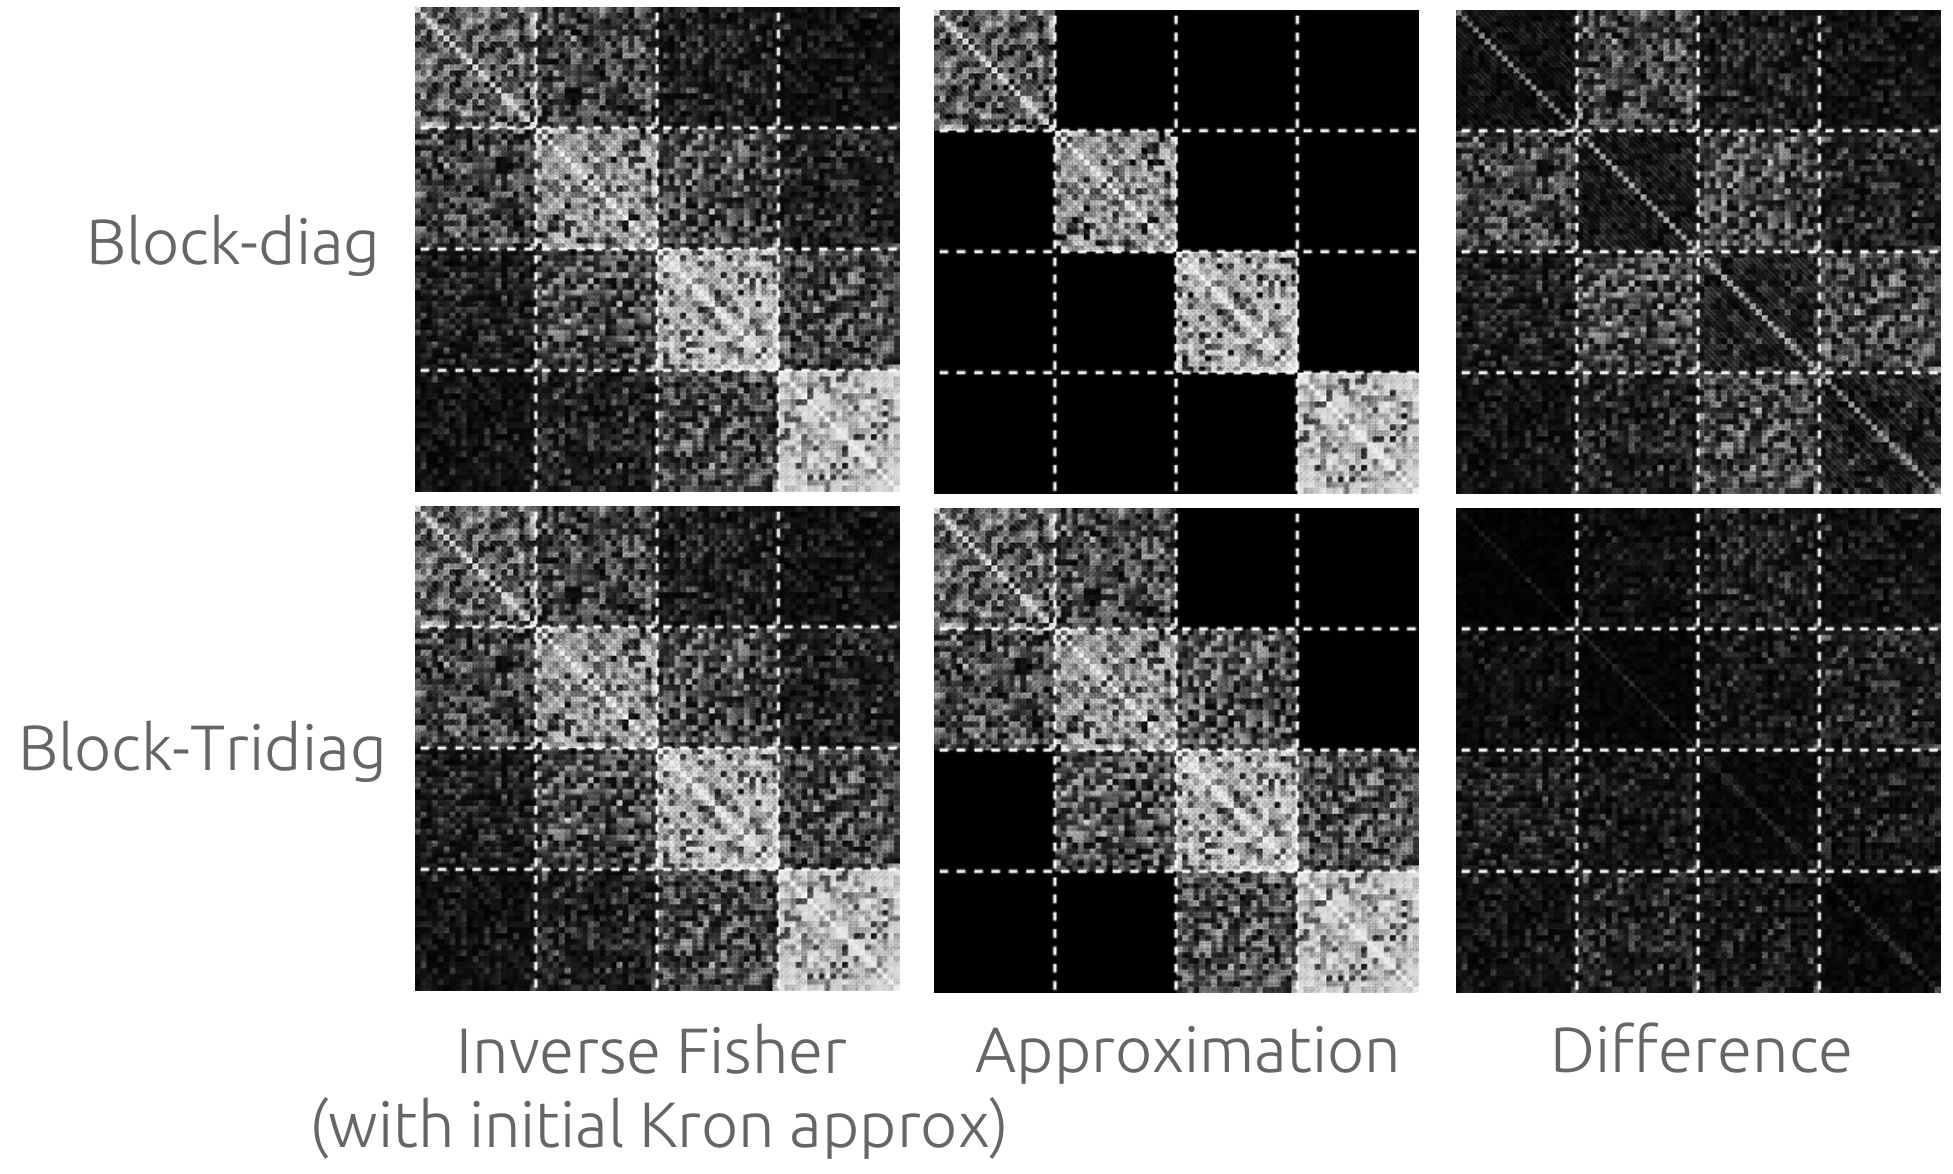
\includegraphics[scale=0.175]{kfac_12}
\end{figure}

\end{frame}

\begin{frame}
\frametitle{KFAC: Block-tridiagonal inverse approx, $\hat{F}^{-1} \approx \tilde{F}^{-1}$}
\begin{itemize}
    \item Define $\hat{F}$ to be the matrix which agrees with $\tilde{F}$ on the tridiagonal blocks, and
        which satisfies the property that $\hat{F}^{-1}$ is block-tridiagonal
    \item Assume that $\hat{F}^{-1}$ is block-tridiagonal is equivalent to
        \begin{itemize}
        \item assuming that it is the precision matrix of an undirected Gaussian graphical model (UGGM) over $\mathcal{D}\theta$
        \end{itemize}
    \item As this graphical model has a tree structure, there is an equivalent
        directed graphical model with the same distribution
        \begin{itemize}
        \item this equivalent directed model will also be linear/Gaussian, and
        \item hence, a directed Gaussian Graphical model (DGGM).
        \end{itemize}
\end{itemize}

{\footnotesize
Recall: The precision matrix of a random vector is the inverse of its covariance matrix.
% * https://www.statlect.com/glossary/precision-matrix
}
\end{frame}

\begin{frame}
\frametitle{KFAC: Block-tridiagonal inverse approx, $\hat{F}^{-1} \approx \tilde{F}^{-1}$}
\begin{figure}
    \centering
    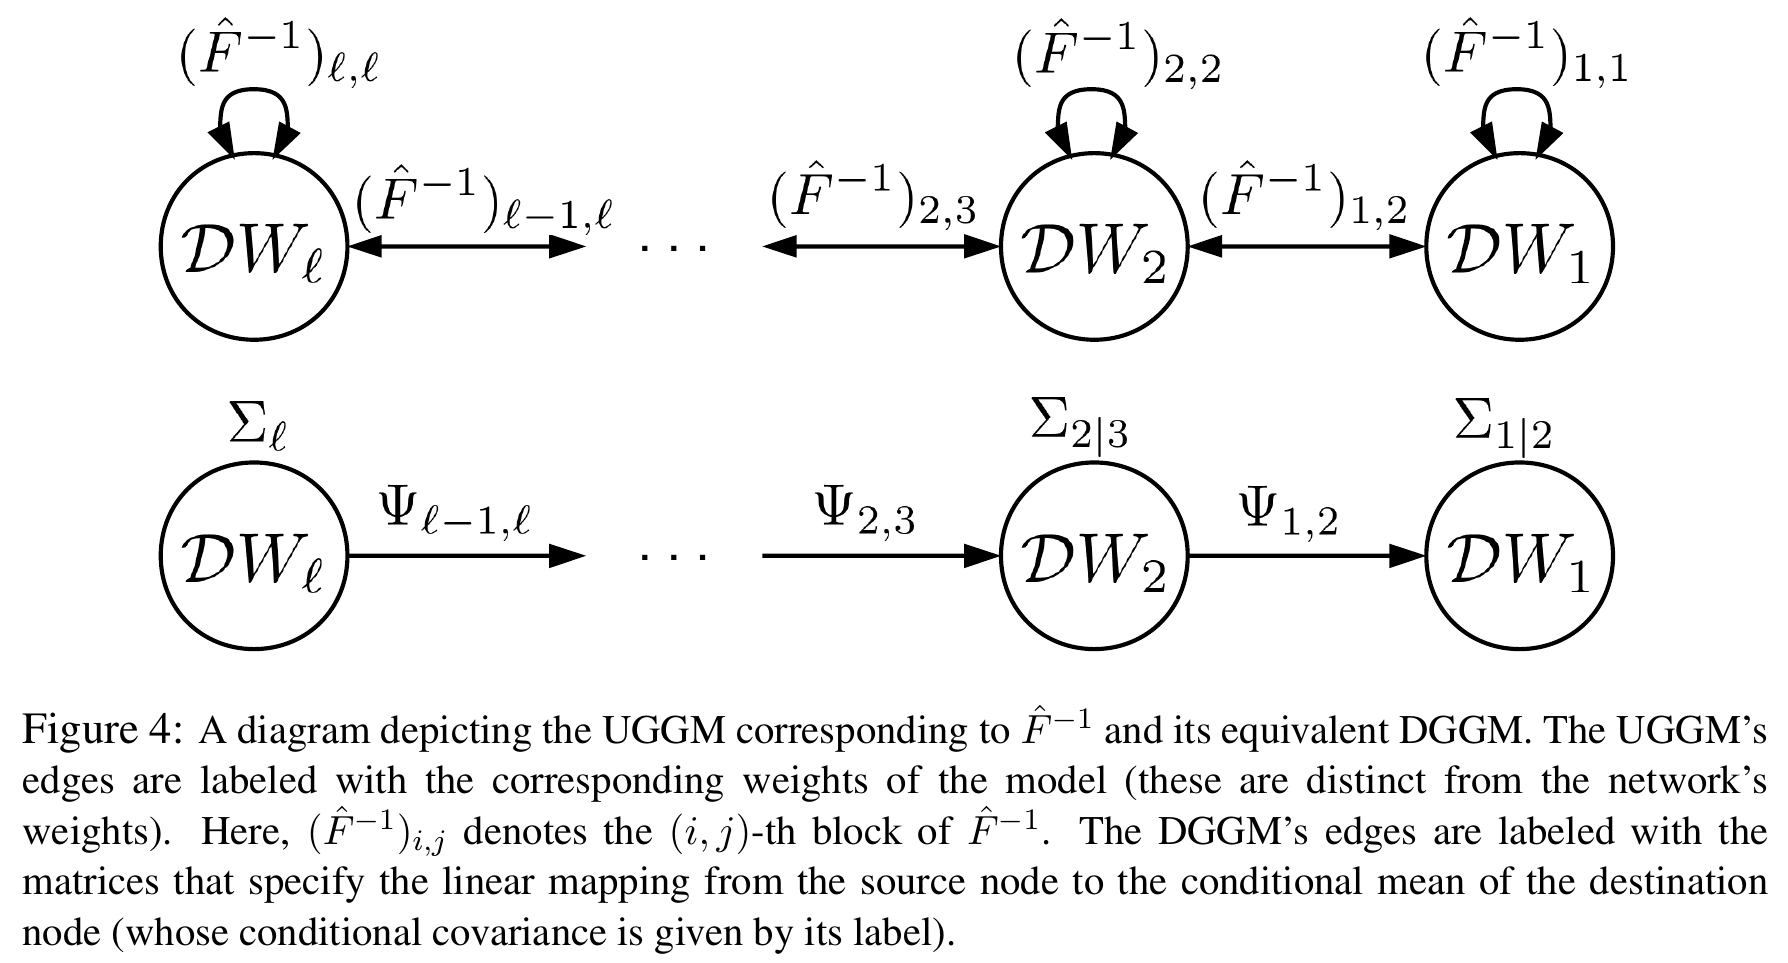
\includegraphics[scale=0.25]{kfac_fig_04_arxiv}
\end{figure}
\end{frame}

\begin{frame}
\frametitle{KFAC: Block-tridiagonal inverse approx, $\hat{F}^{-1} \approx \tilde{F}^{-1}$}
Applying formula for inverse covariance of directed model used in FActorized Natural Gradient (FANG)(Grosse and Salakhutdinov, 2015)
gives:

\begin{figure}
    \centering
    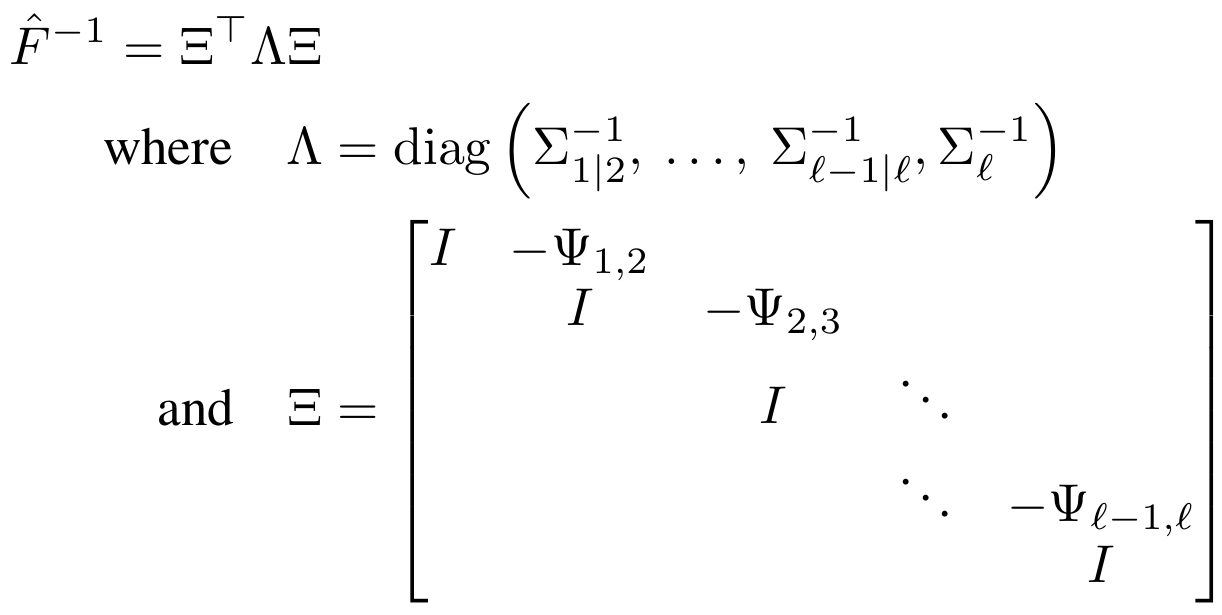
\includegraphics[scale=0.25]{kfac_14}
\end{figure}

% \begin{figure}
%     \centering
%     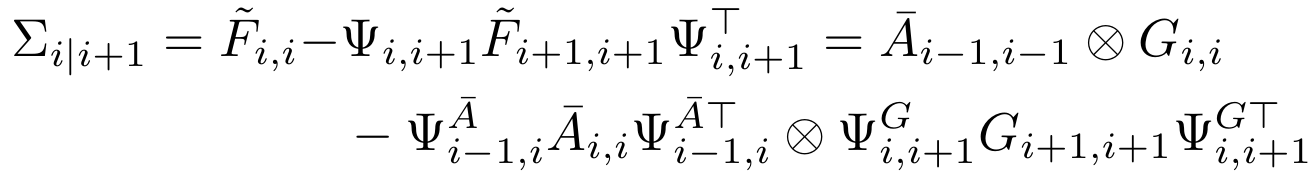
\includegraphics[scale=0.15]{kfac_15}
% \end{figure}
\end{frame}

% \begin{frame}
% \frametitle{KFAC: Block-tridiagonal inverse approx, $\hat{F}^{-1} \approx \tilde{F}^{-1}$}
% \begin{figure}
%     \centering
%     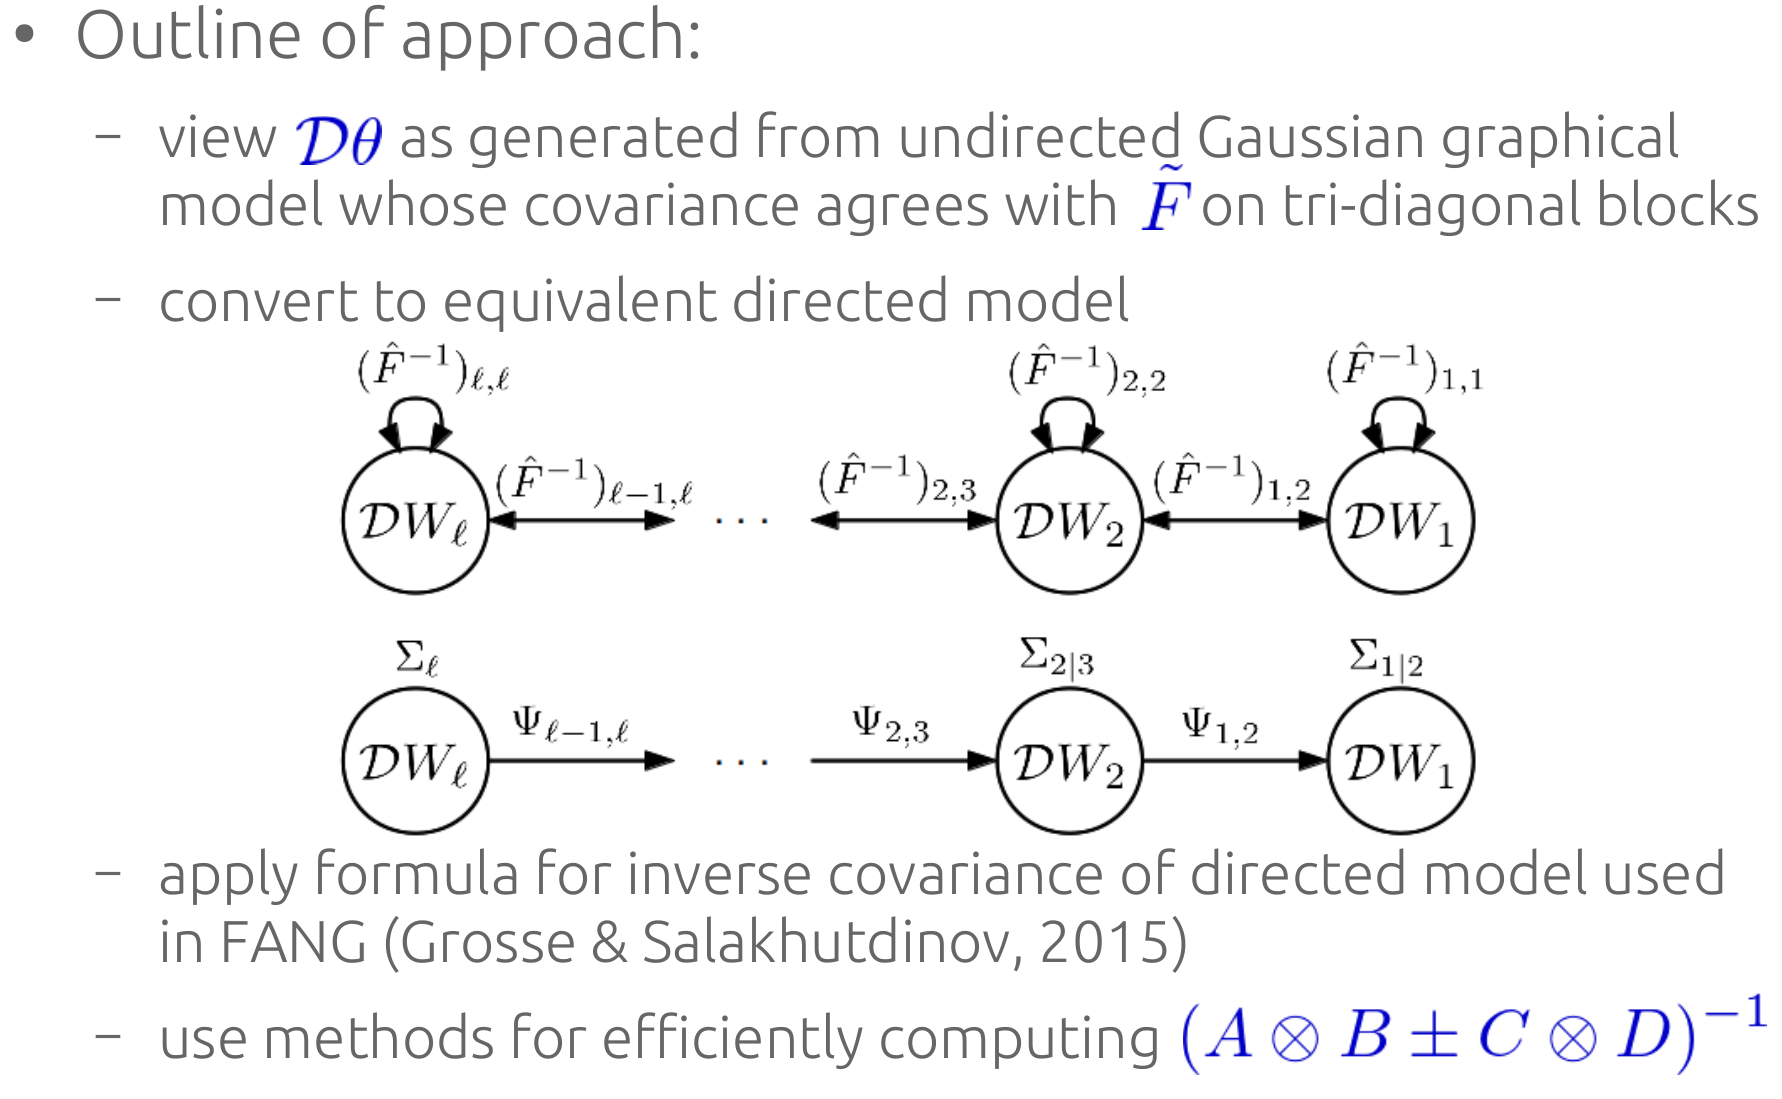
\includegraphics[scale=0.225]{kfac_11}
% \end{figure}
% \end{frame}


\section{Experiments}
\frame{\tableofcontents[currentsection, hideothersubsections]}

\begin{frame}
\frametitle{Experiments}
Setup:
\begin{itemize}
    \item tasks: 3 deep autoencoders: MNIST, FACES, CURVES
    \item baseline: SGD w/ momentum (well-tuned)
    \item $m$ is the mini-batch size;\\
          using an exponentially increasing schedule for $m$, ie
          $m_k = min(1000~exp((k - 1)/b), |S|)$,\\
            $b$ is chosen so that $m_{500} = |S|$ with the sample set $S$
    \item report the results on the training set \\
          (focus on optimization speed, NOT the generalization in the test set)
\end{itemize}
% \begin{figure}
%     \centering
%     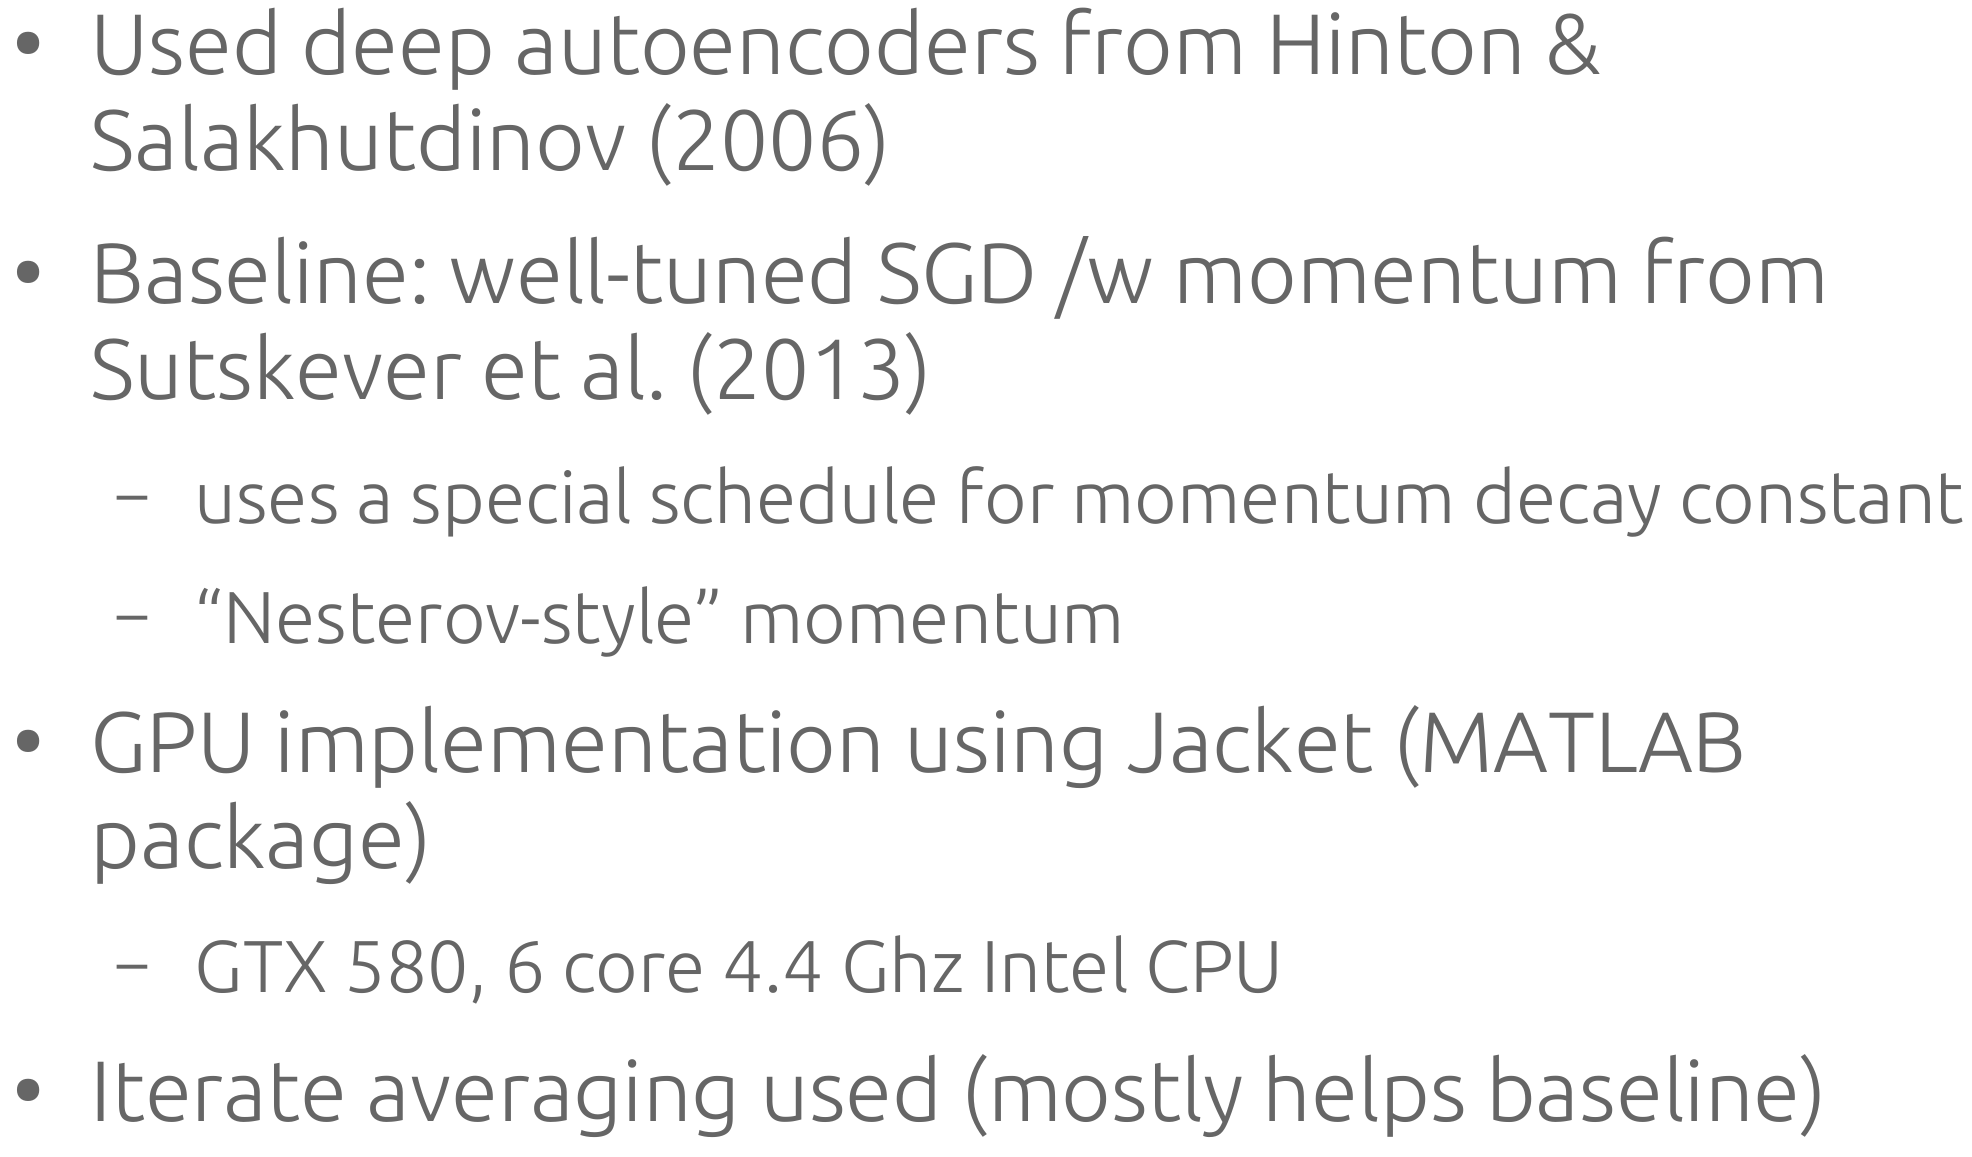
\includegraphics[scale=0.225]{xprmt_setup}
% \end{figure}
\end{frame}

\begin{frame}
\frametitle{Experiments}
\begin{figure}
    \centering
    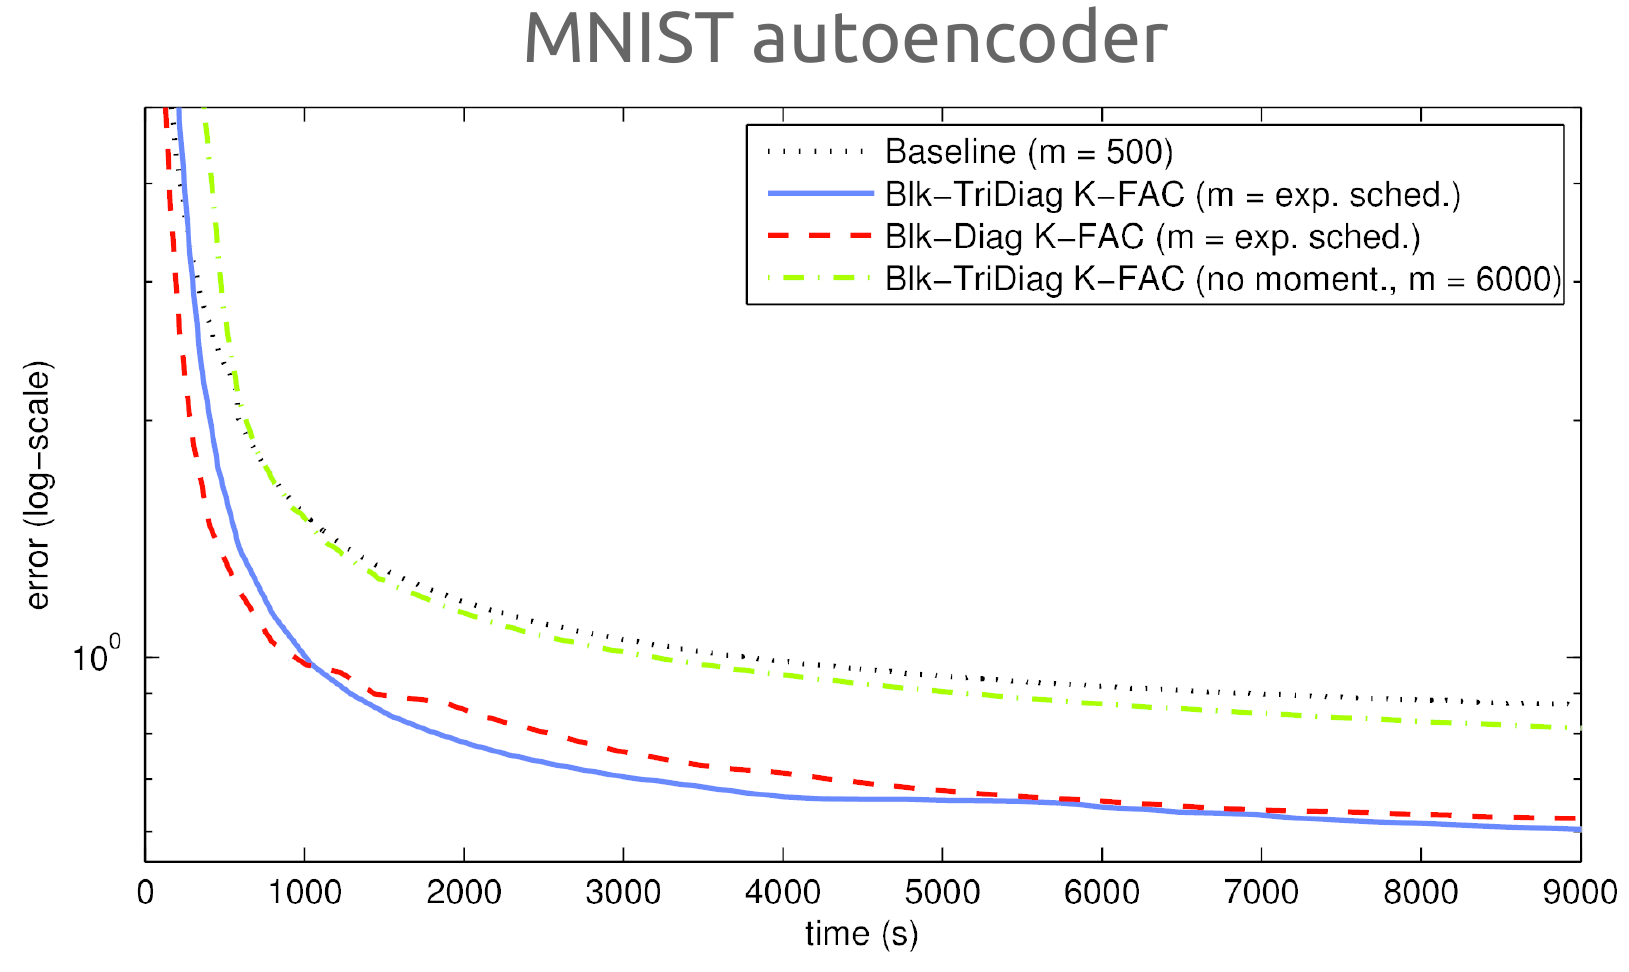
\includegraphics[scale=0.275]{mnist_autoencoder}
\end{figure}
Note: momentum and minibatch size scheduling are crucial!
\end{frame}

\begin{frame}
\frametitle{Experiments}
\begin{figure}
    \centering
    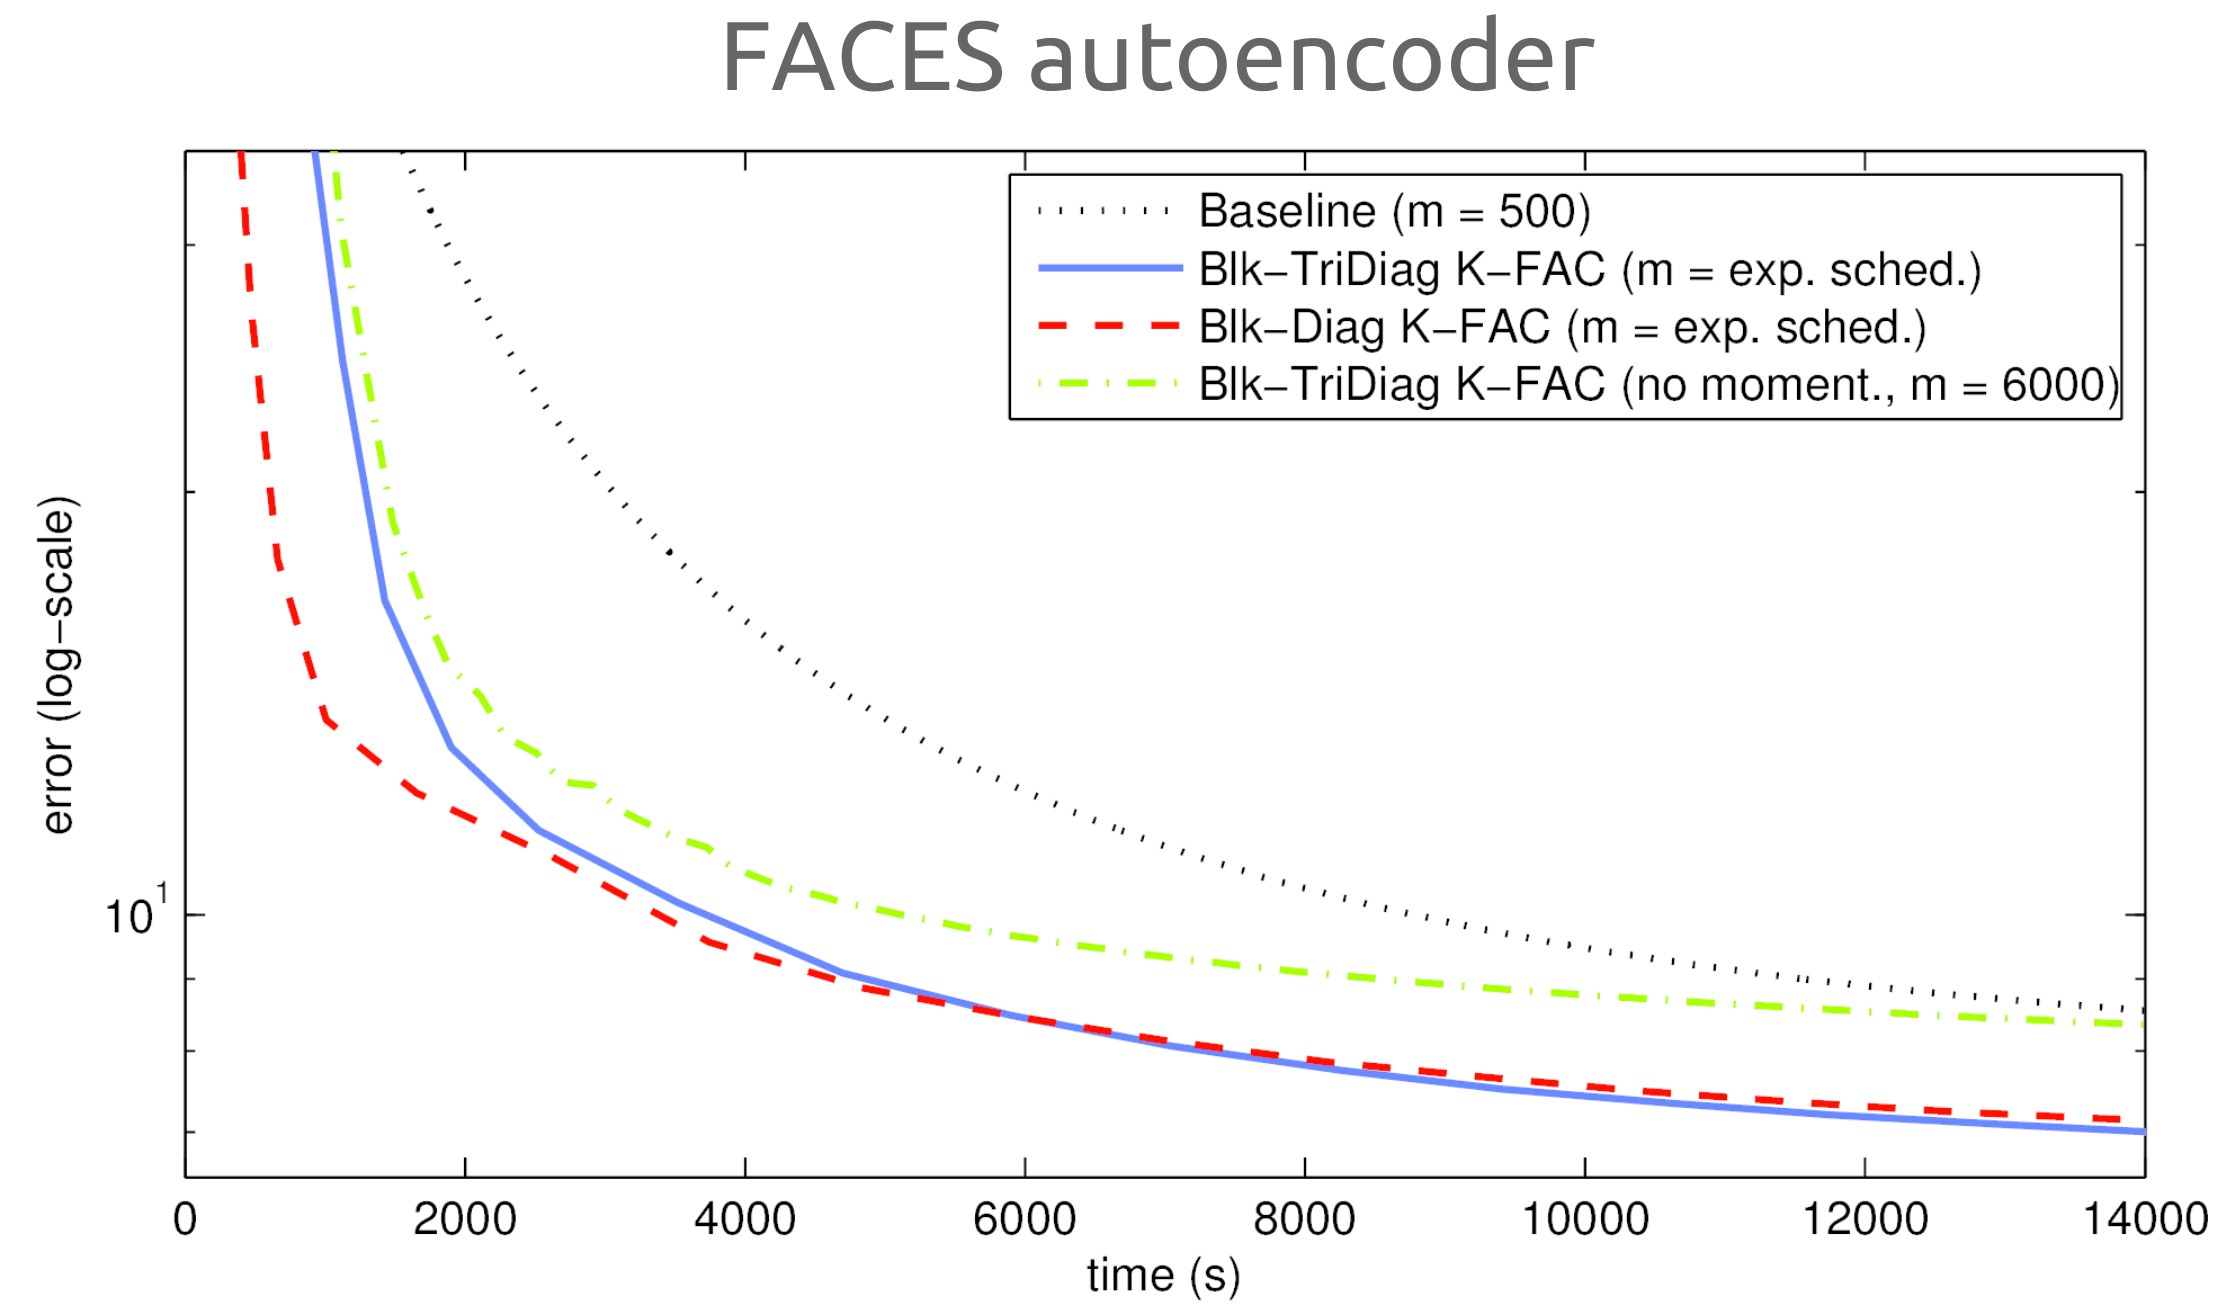
\includegraphics[scale=0.175]{faces_autoencoder}
\end{figure}
Note: the block-diagonal approx is good enough already :), \\
compared to the more sophisticated block-tridiagonal approx!
\end{frame}

\section{Closure}
\frame{\tableofcontents[currentsection, hideothersubsections]}

\begin{frame}
\frametitle{Closure}
{\footnotesize

Skipped parts:
\begin{itemize}
\item Interpretations of approximation
\item Structured inverses (Pourahmadi, 2011)
\item Invariance properties and the relationship to whitening and centering
\item The efficiency improvements, eg damping, momentum, etc
\end{itemize}

Other resources on KFAC:
\begin{itemize}
\item \url{https://arxiv.org/abs/1503.05671} (58-page version)
\item \url{http://www.cs.toronto.edu/~jmartens/docs/KFAC3-MATLAB.zip}
\item \url{https://github.com/tensorflow/kfac} (several in Pytorch, but not official)
\end{itemize}

Follow up:
\begin{itemize}
\item Roger Grosse et al: A Kronecker-factored approximate Fisher matrix for convolution layers. ICML 2016.
\item Yuhuai Wu, et al: Scalable trust-region method for deep reinforcement learning using Kronecker-factored approximation. NIPS 2017.
\item Jimmy Ba, et al: Distributed second-order optimization using Kronecker-factored approximations. ICLR 2017.
\end{itemize}

}
\end{frame}


\begin{frame} [allowframebreaks]
\frametitle{References}
{\tiny
\bibliographystyle{apacite}
\bibliography{ref}
}
\end{frame}

\begin{frame}
\Huge{\centerline{Discussion time and thank you.}}
\end{frame}

%%%%%%%%%%%%%%%%%%%%%%%%%%%%%%%%%%%%%%%%%%%%%%%%%%%%%%%%%%%%%%%%%%%%%%%%%%%%%%%

\end{document}
